\documentclass[11pt]{article}

\usepackage[T1]{fontenc}
\usepackage{lmodern}
\usepackage{microtype}
\usepackage[margin=1in]{geometry}
\usepackage{amsmath,amssymb,amsthm,mathtools}
\usepackage{booktabs,longtable,array}
\usepackage{enumitem}
\usepackage{xcolor}
\usepackage{listings}
\usepackage{graphicx}
\usepackage{mathrsfs}
\usepackage[hidelinks]{hyperref}
\usepackage[nameinlink,capitalise,noabbrev]{cleveref}
\usepackage{fancyhdr}

\definecolor{deepblue}{RGB}{20,55,100}
\definecolor{softgray}{RGB}{245,247,250}
\definecolor{darkred}{RGB}{120,25,25}

\hypersetup{
  pdftitle={Binary Carry Structure in Iterated Lacunary Series},
  pdfauthor={Research note prepared for Vladimir Reshetnikov with OpenAI},
  pdfsubject={OEIS A168362, formal power series iteration, congruences modulo 4},
  pdfkeywords={OEIS A168362, iteration, lacunary series, modulo 4, Lucas theorem}
}

\pagestyle{fancy}
\fancyhf{}
\fancyhead[L]{\small Binary carry structure in iterated lacunary series}
\fancyhead[R]{\small \thepage}
\renewcommand{\headrulewidth}{0.4pt}

\newtheorem{theorem}{Theorem}[section]
\newtheorem{lemma}[theorem]{Lemma}
\newtheorem{proposition}[theorem]{Proposition}
\newtheorem{corollary}[theorem]{Corollary}
\newtheorem{conjecture}[theorem]{Conjecture}
\theoremstyle{definition}
\newtheorem{definition}[theorem]{Definition}
\newtheorem{question}[theorem]{Research question}
\theoremstyle{remark}
\newtheorem{remark}[theorem]{Remark}

\newcommand{\Ftwo}{\mathbb F_2}
\newcommand{\Zfour}{\mathbb Z/4\mathbb Z}
\newcommand{\coef}[2]{[x^{#1}]\,#2}
\newcommand{\wt}{\operatorname{wt}_2}
\newcommand{\band}{\mathbin{\&}}
\newcommand{\bor}{\mathbin{\vert}}
\newcommand{\xor}{\mathbin{\triangle}}
\newcommand{\ind}{\mathbf 1}
\newcommand{\Oh}{\mathrm O}
\newcommand{\circiter}[2]{#1^{\circ #2}}
\newcommand{\MS}{M_s}

% batch 114: cleveref names for the environments sharing the theorem counter
% (until batch 114 every one of them was referred to as ``Theorem'')
\crefname{question}{Research question}{Research questions}
\crefname{conjecture}{Conjecture}{Conjectures}
\AddToHook{env/lemma/begin}{\crefalias{theorem}{lemma}}
\AddToHook{env/proposition/begin}{\crefalias{theorem}{proposition}}
\AddToHook{env/corollary/begin}{\crefalias{theorem}{corollary}}
\AddToHook{env/conjecture/begin}{\crefalias{theorem}{conjecture}}
\AddToHook{env/definition/begin}{\crefalias{theorem}{definition}}
\AddToHook{env/question/begin}{\crefalias{theorem}{question}}
\AddToHook{env/remark/begin}{\crefalias{theorem}{remark}}
% Part II (batch 114)
\newcolumntype{L}[1]{>{\raggedright\arraybackslash}p{#1}}
\newcommand{\Z}{\mathbb Z}
\newcommand{\Q}{\mathbb Q}
\newcommand{\N}{\mathbb N}
\newcommand{\Fp}{\mathbb F_p}
\newcommand{\Zp}{\mathbb Z_p}
\newcommand{\vp}{v_p}
\newcommand{\spn}{s_p}
\newcommand{\itp}[1]{F_p^{\circ #1}}
\newcommand{\A}{A_p}
\newcommand{\Cp}{\mathcal C_p}
\newcommand{\Tp}{\mathcal T_p}
\newcommand{\Hur}{\mathcal H}
\newcommand{\Lfun}{\mathcal L_p}
\DeclareMathOperator{\ord}{ord}

\lstset{
  basicstyle=\ttfamily\small,
  columns=fullflexible,
  frame=single,
  backgroundcolor=\color{softgray},
  breaklines=true,
  showstringspaces=false
}

\title{\bfseries\color{deepblue}
Binary Carry Structure in Iterated Lacunary Series\\[5pt]
\large A complete modulo-four theorem for OEIS A168362,\\
an exact exception criterion, and a logarithmic counting law}
\author{Research note prepared for Vladimir Reshetnikov with OpenAI}
\date{October 1, 2026}

\begin{document}
\maketitle

\begin{abstract}
Let
\[
  F(x)=\sum_{j\ge 0}x^{2^j}=x+x^2+x^4+x^8+\cdots,
  \qquad G_m(x)=F^{\circ m}(x),
\]
and let OEIS A168362 be
\[
  a(n)=\coef{n}{G_n(x)}.
\]
The OEIS entry records two 2026 conjectural observations: the ratio
$a(n+1)/a(n)\sim en$, and a sparse pattern for $a(n)\bmod 4$.  This paper
settles the second observation completely and strengthens it from the diagonal
to the entire iteration array.

The main structural result is that
\[
  \coef{N}{G_m(x)}\equiv0\pmod4
  \qquad\text{whenever }\wt(N)\ge3,
\]
for every $m,N\ge1$, where $\wt(N)$ is the number of $1$'s in the binary
expansion of $N$.  The coefficients at powers of two and at sums of two powers
of two are then described by exact finite bit formulas.  Specializing to the
diagonal gives a complete classification.  Besides the four initial
exceptions $2,3,4,6$, write $n=2^r+2^s$ with $r>s\ge1$ and $d=r-s$.
For $r\ge3$, one has $a(n)\equiv2\pmod4$ precisely when
$d\bmod 2^s$ belongs to an explicitly computable residue set $R_s$.
The first exceptions are
\[
2,3,4,6,20,24,40,68,136,260,520,1028,1032,2056,2064,\ldots.
\]
Thus the theorem confirms every exception printed in the OEIS entry and
predicts all subsequent ones.

Finally, if $E(X)$ counts the exceptional indices up to $X$, then
\[
 E(X)=\kappa\log_2X+\Oh\bigl((\log\log X)^3\bigr),
 \qquad
 \kappa=\sum_{s\ge1}\frac{|R_s|}{2^s}
       =2.323930059308106\ldots.
\]
All finite calculations in the article are reproduced by a standard-library
Python verifier included with the source archive.  The argument itself is
symbolic and does not depend on the computation.
\end{abstract}

\begin{center}
\fbox{\begin{minipage}{0.92\textwidth}
\textbf{Status and proof boundary.}
This is an AI-assisted, unrefereed research manuscript.  The congruence
statements are proved in the text.  The accompanying program independently
checks direct truncated composition modulo $4$ through degree and iterate
$256$, checks the published initial terms, and regenerates all residue tables.
No claim of formal verification in Lean or of publication priority is made.
Independent mathematical review is recommended before an OEIS submission.

\smallskip
[Write note, batch 73O1: filed in ProveIt's research-report collection;
provenance and status in \cref{lim:sec:collection}.]
\end{minipage}}
\end{center}

\emph{[Write note, batch 114, 6 October 2026.]} Since batch~114 the report has two Parts. Part~I
(Sections~1--14 and Appendices~A--B) is the report described above,
unchanged except for the Part headings and dated notes. Part~II
(\cref{lim:dsd:sec:front}; Sections~15--27 and
Appendices~\ref{lim:dsd:app:oeis-note}--\ref{lim:dsd:app:inventory}) adds
the manuscript \emph{Digit-Sum Divisibility in Lacunary Iteration}
(5~October 2026): for every prime $p$ and every integer iterate $m$,
inverse iterates included, the coefficients of $F_p^{\circ m}$, where
$F_p=\sum_jx^{p^j}$, satisfy $v_p([x^N]F_p^{\circ m})\ge(s_p(N)-1)/(p-1)$.
It answers Research question~\ref{lim:q:higher-precision}, re-scopes
Research question~\ref{lim:q:odd-prime}, and proves
\cref{lim:thm:whole-array-support,lim:prop:P-closed,lim:prop:diagonal-even}
again at $p=2$ as special cases. Its labels carry the prefix
\texttt{lim:dsd:}. The write also corrected the names of
cross-references: until batch~114 every lemma, proposition, corollary,
definition, conjecture, remark and research question of Part~I was cited
as a ``Theorem'' (for example ``Summing Theorem~3.1'' for
\cref{lim:lem:balanced-pairs}); each is now cited by its own name. No
number changed.

\tableofcontents

\part{The modulo-four theorem: binary carry structure}


\section{The OEIS problem and the new results}

The sequence A168362 is defined by the main diagonal of the iteration table of
$F(x)=\sum_{j\ge0}x^{2^j}$:
\begin{equation}\label{lim:eq:def-a}
  a(n)=\coef{n}{F^{\circ n}(x)}.
\end{equation}
Its initial values are
\[
1,2,6,34,280,3010,39984,634040,11704548,\ldots.
\]
The current OEIS entry records the conjectural ratio
\begin{equation}\label{lim:eq:ratio-conj}
  \frac{a(n+1)}{a(n)}\sim en
\end{equation}
and the observed congruence pattern
\begin{equation}\label{lim:eq:oeis-mod4-observation}
  a(n)\equiv2\pmod4
  \quad\text{at }n=2,3,4,6,20,24,40,68,136,260,520,\ldots,
\end{equation}
with apparent divisibility by $4$ elsewhere; see~\cite{OEIS-A168362}.

The purpose of this article is arithmetic rather than asymptotic.  The ratio
problem~\eqref{lim:eq:ratio-conj} remains open here.  The modulo-four observation,
however, is completely resolved.  The result is stronger than a list of
indices: it gives a short bitwise decision procedure, describes every entry of
the two-dimensional iteration table modulo $4$, and yields an asymptotic law
for the number of exceptions.

\subsection{Statement of the diagonal classification}

For nonnegative integers $u,v$, $u\band v$ and $u\bor v$ denote bitwise AND
and OR.  Let $\wt(u)$ be the binary Hamming weight.  For $s\ge1$, put
$M_s=2^s-1$ and define a subset $R_s\subseteq\mathbb Z/2^s\mathbb Z$ by
\begin{equation}\label{lim:eq:R-def-intro}
\ind_{d\in R_s}
 \equiv
 \ind_{d\equiv0\ (2^s)}
 +\sum_{i=0}^{s}
   \ind_{\,i\bor((i+d)\bmod2^s)=M_s}
 \pmod2.
\end{equation}
This is an exact finite definition involving only $s+2$ Boolean tests.

\begin{theorem}[Complete modulo-four classification for A168362]
\label{lim:thm:diagonal-classification}
For $n>1$, $a(n)$ is even.  Moreover, $a(n)\equiv2\pmod4$ if and only if
one of the following holds:
\begin{enumerate}[label=\textup{(\roman*)}]
  \item $n\in\{2,3,4,6\}$;
  \item $n=2^r+2^s$ with $r>s\ge1$, $r\ge3$, and
        $r-s\pmod{2^s}\in R_s$.
\end{enumerate}
Every other $n>1$ satisfies $a(n)\equiv0\pmod4$.
\end{theorem}

The residue sets begin
\begin{align*}
R_1&=\varnothing,\\
R_2&=\{0,2\},\\
R_3&=\{0,1,2,4,6,7\},\\
R_4&=\{0,7,9,10,11,12,14,15\},\\
R_5&=\{0,21,22,23,27,28,30,31\},\\
R_6&=\{0,51,54,57,59,60,62,63\}.
\end{align*}
For example, $s=2$ gives the particularly simple family
\[
  a(2^r+4)\equiv2\pmod4
  \quad\Longleftrightarrow\quad r\text{ is even},
  \qquad r\ge3.
\]
This produces $20,68,260,1028,4100,16388,\ldots$.

\emph{[Write note, batch 73O1.]} Since $R_1=\varnothing$, case~(ii) of
\cref{lim:thm:diagonal-classification} never holds with $s=1$: the
exceptional two-bit indices all have $s\ge2$. The condition is stated as
$r>s\ge1$ in the source and is kept.

\subsection{A theorem for the whole iteration array}

The diagonal theorem follows from a more general statement.  Write
\begin{equation}\label{lim:eq:gmn}
  g_m(N)=\coef{N}{G_m(x)},\qquad G_m(x)=F^{\circ m}(x).
\end{equation}

\begin{theorem}[Binary-weight support modulo four]
\label{lim:thm:whole-array-support}
For every $m,N\ge1$,
\[
  \wt(N)\ge3\quad\Longrightarrow\quad g_m(N)\equiv0\pmod4.
\]
In addition, $g_m(N)$ is odd only when $N$ is a power of two.  Exact formulas
for the remaining one-bit and two-bit exponents are given in
\Cref{lim:thm:full-array-formula}.
\end{theorem}

\emph{[Write note, batch 114, 6 October 2026.]} Part~II proves $2^{s_2(N)-1}\mid[x^N]F^{\circ m}(x)$ for every
$N\ge1$ and every integer $m$, inverse iterates included
(\eqref{lim:dsd:eq:binary-main}, the case $p=2$ of \cref{lim:dsd:thm:main}).
Since $s_2(N)=\wt(N)$, this contains both assertions of the theorem, by a
different route (scaling to integral exponential series and Legendre's
formula, with no carry calculus; write note in \cref{lim:dsd:sec:class}),
and it holds modulo every $2^q$. The exact formulas of
\cref{lim:thm:full-array-formula} are not proved again there.

This support theorem is not a numerical coincidence.  It is a consequence of
the fact that, modulo $4$, the only cross terms that survive a $2^k$-th power
are balanced products of two monomials.  That two-adic fact is the core of the
proof.

\subsection{Place in the ProveIt collection}
\label{lim:sec:collection}

\emph{[Write note, batch 73O1, 1 October 2026.]} This report is filed in
ProveIt's research-report collection, in the directory
\begin{center}\small
\nolinkurl{SetTheory/Cardinals/docs/reports/congruences-and-valuations/}\\
\nolinkurl{iterated-series/a168362-lacunary-iterates-mod4}.
\end{center}
Its README there is the guide to the files.

\emph{Provenance.} The report is built from one manuscript: manuscript~49
of batch~73 (cluster O1) of ProveIt's incoming-reports intake, the archive
\texttt{ProveIt\_A168362\_Mod4\_Theorem.zip}, which arrived in commit
\texttt{3a9518c52} and was placed by commit \texttt{9df4ba51a}. The
manuscript names no pinned commit; it says the repository~\cite{ProveIt}
was inspected on 1 October 2026. The text is printed as delivered. The
write changed only the label names, which now carry the prefix
\texttt{lim:}, and added the notes marked \emph{[Write note]}. Nothing was
merged into it; no other manuscript of the batch treats this sequence.
The delivered bibliography also lists two general references, on formal
power series~\cite{StanleyEC1} and on analytic
combinatorics~\cite{FlajoletSedgewick}, which the delivered text never
cites; they are kept as background.

\emph{Status.} The manuscript was prepared with OpenAI. It is unrefereed,
and nothing in it is formalized in Lean or any other proof assistant. The
intake reran the shipped verifier on a copy (exit code~0; the three data
files it writes equal the shipped ones, up to line endings). Independently
of the delivered code, it composed $F$ modulo~$4$ to degree and iterate
$1100$: the diagonal exceptions are $2,3,4,6,20,24,40,68,136,260,520,1028,1032$,
as \cref{lim:thm:diagonal-classification} predicts, and
\cref{lim:thm:whole-array-support} holds for $m\le300$, $N\le1100$. It
also recomputed $a(1),\ldots,a(10)$, the sets $R_1,\ldots,R_8$, the tail
bound of the series for $\kappa$, and the row $n=20$ of
\cref{lim:tab:ratio-data}. It did not re-derive every proof. The OEIS
statements quoted here (the comments of 22 May 2026 on A168362, and the
entries A112317, A122888 and A086753) were confirmed on the live entries on
1 October 2026.

\emph{Neighbouring reports.} In the same collection:
\begin{itemize}
\item the two other reports in \texttt{iterated-series} prove congruences
  for compositional iterates of other series:\newline
  \texttt{a396807-self-iterating-series} and\newline
  \texttt{compositional-tree-series-congruences};
\item \texttt{a000139-binary-carries-parity} uses the same binary-carry
  (Kummer--Lucas) technique for a different sequence.
\end{itemize}
There is no overlap, and no statement here depends on them.

\section{Formal-series setup and binary lifts}

All power series below have zero constant term, so formal composition is
well-defined.  We work coefficientwise; therefore every assertion remains
valid after truncation to any finite degree.

For a binary series $P=\sum p_nx^n\in\Ftwo[[x]]$, let
\[
  [P]=\sum \widetilde p_nx^n\in\Zfour[[x]]
\]
denote the canonical lift, where $\widetilde p_n\in\{0,1\}$.  Every series
$H\in\Zfour[[x]]$ has a unique binary decomposition
\begin{equation}\label{lim:eq:binary-decomposition}
  H=[P]+2[Q],\qquad P,Q\in\Ftwo[[x]].
\end{equation}
The first component records coefficient parity, while the second records the
next binary digit.

Let $T$ be Frobenius on $\Ftwo[[x]]$:
\[
  T(P)=P^2.
\]
Because the characteristic is two,
\[
  F(P)=P+P^2+P^4+\cdots=(1+T)^{-1}P.
\]
Here the inverse is the coefficientwise convergent geometric series
$1+T+T^2+\cdots$.

\section{The modulo-four polarization identity}

\subsection{A multinomial valuation lemma}

\begin{lemma}[Only balanced pairs survive]
\label{lim:lem:balanced-pairs}
Let $z_1,z_2,\ldots$ be commuting indeterminates of positive degree.  For
$k\ge1$,
\begin{equation}\label{lim:eq:balanced-pairs}
 \left(\sum_j z_j\right)^{2^k}
 \equiv
 \sum_j z_j^{2^k}
 +2\sum_{i<j}(z_iz_j)^{2^{k-1}}
 \pmod4.
\end{equation}
\end{lemma}

\begin{proof}
Consider a multinomial term with exponents $e_1,e_2,\ldots$ summing to $2^k$.
Legendre's formula gives
\[
 v_2\!\left(\frac{(2^k)!}{\prod_j e_j!}\right)
 =\sum_j s_2(e_j)-1,
\]
where $s_2$ is binary digit sum.  The valuation is zero exactly when one
$e_j=2^k$ and all other exponents vanish.  The valuation is one exactly when
the total binary digit sum of the nonzero exponents is two.  Since their sum is
a single power of two, this forces exactly two nonzero exponents, both equal to
$2^{k-1}$.  Every other multinomial coefficient is divisible by $4$.
The balanced binomial coefficient has valuation one, hence is congruent to
$2$ modulo $4$.  This proves~\eqref{lim:eq:balanced-pairs}.
\end{proof}

\subsection{Polarizing the lacunary operator}

Summing \Cref{lim:lem:balanced-pairs} over $k$ gives a compact identity.

\begin{corollary}[Lacunary polarization]
\label{lim:cor:lacunary-polarization}
For positive-degree monomials $z_j$,
\begin{equation}\label{lim:eq:lacunary-polarization}
 F\!\left(\sum_jz_j\right)
 \equiv
 \sum_jF(z_j)+2\sum_{i<j}F(z_iz_j)
 \pmod4.
\end{equation}
\end{corollary}

A second elementary fact explains how the $2[Q]$ component propagates.

\begin{lemma}[The high binary digit is carried unchanged]
\label{lim:lem:q-passes}
For $P,Q\in\Ftwo[[x]]$,
\begin{equation}\label{lim:eq:q-passes}
  F([P]+2[Q])\equiv F([P])+2[Q]\pmod4.
\end{equation}
\end{lemma}

\begin{proof}
The term with exponent one is $[P]+2[Q]$.  For every $k\ge1$,
$([P]+2[Q])^{2^k}\equiv[P]^{2^k}\pmod4$, because every term containing
$2[Q]$ has a factor divisible by $4$.
\end{proof}

\section{The carry transform}

The parity iterates are supported only on powers of two.  It is therefore
useful to encode a subset $S\subseteq\mathbb Z_{\ge0}$ by
\[
  P_S(x)=\sum_{j\in S}x^{2^j}\in\Ftwo[[x]].
\]
For $r\ge0$, define the prefix count
\[
  N_S(r)=|S\cap\{0,1,\ldots,r\}|.
\]

\begin{definition}[Carry transform]
\label{lim:def:carry-transform}
The binary series $\mathcal C(P_S)$ is defined by
\begin{align}
 \coef{2^r}{\mathcal C(P_S)}
   &=\binom{N_S(r)}2\pmod2,
   \label{lim:eq:carry-one-bit}\\
 \coef{2^r+2^s}{\mathcal C(P_S)}
   &=\sum_{i=0}^{s}\ind_{i\in S}\ind_{i+r-s\in S}\pmod2,
   \qquad r>s,
   \label{lim:eq:carry-two-bit}
\end{align}
and all coefficients at exponents of binary weight at least three are zero.
\end{definition}

\begin{proposition}[Exact lift of one lacunary step]
\label{lim:prop:one-step-lift}
For every $S$,
\begin{equation}\label{lim:eq:one-step-lift}
  F([P_S])\equiv [F(P_S)]+2[\mathcal C(P_S)]\pmod4.
\end{equation}
\end{proposition}

\begin{proof}
By \Cref{lim:cor:lacunary-polarization},
\[
 F([P_S])\equiv
 \sum_{j\in S}F(x^{2^j})
 +2\sum_{\substack{i<j\\ i,j\in S}}F(x^{2^i+2^j})\pmod4.
\]
At exponent $2^r$, the first sum has coefficient $N_S(r)$.  Its low binary
digit is $N_S(r)\bmod2$, and its next digit is
\[
 \left\lfloor\frac{N_S(r)}2\right\rfloor
 \equiv\binom{N_S(r)}2\pmod2.
\]
This gives~\eqref{lim:eq:carry-one-bit}.  In the second sum, the exponent
$2^r+2^s$ occurs from a pair $(i,j)$ precisely when
$(i,j)=(s-k,r-k)$ for some $0\le k\le s$.  Reindexing by $i=s-k$ gives
\eqref{lim:eq:carry-two-bit}.  No exponent with three binary $1$'s can occur.
\end{proof}

\section{Closed form for the parity iterates}

Write
\begin{equation}\label{lim:eq:PQ-iterates}
  G_m(x)\equiv[P_m(x)]+2[Q_m(x)]\pmod4,
  \qquad P_m,Q_m\in\Ftwo[[x]].
\end{equation}
Starting with $P_0=x$ and $Q_0=0$, \Cref{lim:lem:q-passes,lim:prop:one-step-lift}
give
\begin{equation}\label{lim:eq:PQ-recurrence}
  P_{m+1}=F(P_m),
  \qquad
  Q_{m+1}=Q_m+\mathcal C(P_m)
  \quad\text{in }\Ftwo[[x]].
\end{equation}

\begin{proposition}[Negative-binomial parity formula]
\label{lim:prop:P-closed}
For $m\ge1$,
\begin{equation}\label{lim:eq:P-closed}
  P_m(x)=\sum_{j\ge0}\binom{m+j-1}{j}x^{2^j}
  \quad\text{in }\Ftwo[[x]].
\end{equation}
Equivalently, if
\[
  S_m=\{j\ge0:j\band(m-1)=0\},
\]
then $P_m=P_{S_m}$.
\end{proposition}

\begin{proof}
Over $\Ftwo[[x]]$, $F=(1+T)^{-1}$.  Therefore
\[
 P_m=(1+T)^{-m}x
 =\sum_{j\ge0}\binom{m+j-1}{j}T^jx,
\]
which is~\eqref{lim:eq:P-closed}.  Lucas's theorem, or equivalently the no-carry
form of Kummer's theorem, says that
$\binom{m+j-1}{j}$ is odd exactly when the addition of $j$ and $m-1$ has no
binary carry, namely when $j\band(m-1)=0$; see~\cite{Fine1947}.
\end{proof}

\emph{[Write note, batch 114, 6 October 2026.]} Part~II proves
$A_p(m,p^r)\equiv(-1)^r\binom{-m}{r}\pmod p$ for every prime $p$ and every
$m\in\mathbb Z$ \eqref{lim:dsd:eq:modp-row}, by the same operator argument
with $\tau\colon H(x)\mapsto H(x^p)$ in place of $T$. At $p=2$ and $m\ge1$
this, with the support of $P_m$ at powers of two, is \eqref{lim:eq:P-closed}
(write note in \cref{lim:dsd:sec:consequences}).

Combining the recurrence with the closed form gives the promised theorem for
the complete array.

\begin{theorem}[Exact array formula modulo four]
\label{lim:thm:full-array-formula}
Let $m\ge1$.
\begin{enumerate}[label=\textup{(\alph*)}]
\item If $\wt(N)\ge3$, then $g_m(N)\equiv0\pmod4$.
\item If $N$ is not a power of two, then $g_m(N)$ is even.
\item For $N=2^r$,
\begin{equation}\label{lim:eq:array-power-formula}
 g_m(2^r)\equiv
 \binom{m+r-1}{r}
 +2\sum_{\ell=1}^{m-1}
     \binom{\#\{0\le j\le r:j\band(\ell-1)=0\}}2
 \pmod4.
\end{equation}
\item For $N=2^r+2^s$ with $r>s\ge0$, put $d=r-s$ and
\begin{equation}\label{lim:eq:E-def}
 E(M,B)=\#\{0\le t\le M:t\band B=0\}\pmod2,
 \qquad E(M,B)=0\text{ for }M<0.
\end{equation}
Then
\begin{equation}\label{lim:eq:array-two-bit-formula}
  g_m(2^r+2^s)
  \equiv
  2\sum_{i=0}^{s}E(m-2,\,i\bor(i+d))
  \pmod4.
\end{equation}
\end{enumerate}
\end{theorem}

\begin{proof}
By~\eqref{lim:eq:PQ-recurrence},
$Q_m=\sum_{\ell=0}^{m-1}\mathcal C(P_\ell)$; the $\ell=0$ carry is zero.
Every $P_\ell$ is supported at one-bit exponents, and every
$\mathcal C(P_\ell)$ is supported at exponents of weight at most two.
This proves (a) and (b).  Formula~\eqref{lim:eq:array-power-formula} follows from
\eqref{lim:eq:carry-one-bit} and \Cref{lim:prop:P-closed}.

For a two-bit exponent, substitute $S_\ell$ into
\eqref{lim:eq:carry-two-bit}.  With $t=\ell-1$, membership of both $i$ and $i+d$
in $S_\ell$ is equivalent to
\[
 t\band i=0,
 \qquad t\band(i+d)=0,
\]
and hence to $t\band(i\bor(i+d))=0$.  Summing $0\le t\le m-2$ gives
\eqref{lim:eq:array-two-bit-formula}.
\end{proof}

\emph{[Correction, 6 October 2026, after the independent check of the
batch-114 write.]} Formula~\eqref{lim:eq:array-power-formula} is printed
above as delivered in batch~73O1. Its first term must be read as the
coefficient of $x^{2^r}$ in $[P_m]$, that is, as $\binom{m+r-1}{r}$ reduced
modulo~$2$ to $\{0,1\}$: the proof obtains it from~\eqref{lim:eq:PQ-iterates}
and~\eqref{lim:eq:P-closed}, which determine only that parity. With the
binomial read as an integer, (c) is false. For $m=2$ and $r=1$ the right side
is $\binom21+2\binom22=4\equiv0\pmod4$, while
$g_2(2)=[x^2]\bigl(F(x)+F(x)^2+F(x)^4+\cdots\bigr)=1+1=2$; for $m=3$ and
$r=1$ it is $3+2=5\equiv1$, while $g_3(2)=3$. The repaired statement is
\[
 g_m(2^r)\equiv
 \Bigl(\binom{m+r-1}{r}\bmod2\Bigr)
 +2\sum_{\ell=1}^{m-1}
     \binom{\#\{0\le j\le r:j\band(\ell-1)=0\}}2
 \pmod4,
\]
with $\binom{m+r-1}{r}\bmod2\in\{0,1\}$. An independent computation (exact
composition modulo~$4$ for $1\le m\le6$ and $1\le N\le160$) compared parts
(a)--(d) with $g_m(N)$: with the integer reading, (c) fails at $19$ of the
$960$ entries, all at powers of two; with the reading modulo~$2$, no entry
fails. The proof of \cref{lim:prop:power-diagonal} uses
\eqref{lim:eq:array-power-formula} with this reading: it discards
$\binom{2^r+r-1}{r}$, which is even by \cref{lim:prop:diagonal-even} but
can be $\equiv2\pmod4$ (it is $2$ at $r=1$). So
\cref{lim:prop:power-diagonal} and \cref{lim:thm:diagonal-classification}
stand as stated; parts (a), (b) and (d) are unaffected. No other place in
Part~I or Part~II uses the integer reading: Part~II compares with (c) only
at weight~$0$, where the residue is taken modulo~$2$
(\cref{lim:dsd:sec:claims}), and the delivered verifier
\texttt{code/verify\_a168362.py} tests one-bit exponents only for parity
and on the diagonal $m=N$. Under Vladimir Reshetnikov's standing rule of
4~October 2026 the printed formula is kept, and this note records the
counterexample and the repair.

\begin{remark}[A logarithmic-time evaluation of $E$]
\label{lim:rem:E-fast}
The parity in~\eqref{lim:eq:E-def} can be evaluated without enumeration.  Every
admissible $t\le M$ is either the tight word $t=M$ or has a highest bit $j$ at
which $M_j=1$ and $t_j=0$.  Hence
\begin{equation}\label{lim:eq:E-first-difference}
 E(M,B)=\ind_{M\band B=0}
 \mathbin{\oplus}
 \bigoplus_{\substack{j:M_j=1;\\
   (M\gg(j+1))\band(B\gg(j+1))=0;\\
   B\bmod2^j=2^j-1}}1,
\end{equation}
where $\oplus$ denotes XOR.  Thus every entry at a two-bit exponent is
computable in $\Oh(s\log m)$ bit operations.
\end{remark}

\section{Specialization to the A168362 diagonal}

We now set $m=N=n$.

\subsection{All noninitial diagonal terms are even}

\begin{proposition}[Diagonal parity]
\label{lim:prop:diagonal-even}
For every $n>1$, $a(n)$ is even.
\end{proposition}

\begin{proof}
If $n$ is not a power of two, this follows from
\Cref{lim:thm:full-array-formula}(b).  If $n=2^r$ with $r\ge1$, the parity is
\[
 \binom{2^r+r-1}{r}\pmod2.
\]
By Lucas's theorem it would be odd only if $r\band(2^r-1)=0$.  But
$0<r<2^r$ and the lowest $r$ binary positions of $2^r-1$ are all $1$, so
$r\band(2^r-1)=r\ne0$.
\end{proof}

\emph{[Write note, batch 114, 6 October 2026.]} Part~II's \cref{lim:dsd:cor:diagonal-p} proves
$p\mid A_p(N,N)$ for every prime $p$ and every $N>1$. At $p=2$ it is this
proposition, with a different argument at $n=2^r$ (write note in
\cref{lim:dsd:sec:consequences}).

\subsection{Powers of two}

\begin{proposition}[The one-bit diagonal]
\label{lim:prop:power-diagonal}
For $r\ge1$,
\[
  a(2^r)\equiv2\pmod4
  \quad\Longleftrightarrow\quad r\in\{1,2\}.
\]
Thus only $n=2$ and $n=4$ are exceptional powers of two.
\end{proposition}

\begin{proof}
For $t=0,1,\ldots,2^r-2$, put
\[
 N_t=\#\{0\le j\le r:j\band t=0\}.
\]
By~\eqref{lim:eq:array-power-formula} and \Cref{lim:prop:diagonal-even}, the second
binary digit of $a(2^r)$ is
\[
 \sum_{t=0}^{2^r-2}\binom{N_t}{2}\pmod2.
\]
Interchange the sum over $t$ with the choice of a pair $0\le i<j\le r$:
\begin{equation}\label{lim:eq:power-pair-swap}
 \sum_{0\le i<j\le r}
 \#\{0\le t\le2^r-2:t\band(i\bor j)=0\}\pmod2.
\end{equation}
The excluded value $t=2^r-1$ is never counted because $i\bor j>0$.
Over the complete set of $r$-bit values, the inner count is
$2^{r-\wt(i\bor j)}$, which is odd exactly when $i\bor j=2^r-1$.
For $r=1$, the pair $(0,1)$ works; for $r=2$, the pair $(1,2)$ works.  For
$r\ge3$, both $i$ and $j$ are at most $r<2^{r-1}$, so their OR is smaller
than $2^r-1$.  This proves the claim.
\end{proof}

\subsection{Two-bit exponents}

For $n=2^r+2^s$, $r>s\ge0$, \Cref{lim:thm:full-array-formula} gives the exact
criterion
\begin{equation}\label{lim:eq:q-general-diagonal}
 \frac{a(n)}2
 \equiv
 \sum_{i=0}^{s}E(n-2,\,i\bor(i+r-s))
 \pmod2.
\end{equation}
The following elementary evaluation is what turns this into
\Cref{lim:thm:diagonal-classification}.

\begin{lemma}[A nearly complete binary interval]
\label{lim:lem:nearly-complete}
For $s\ge1$ and $B\ge0$,
\begin{equation}\label{lim:eq:nearly-complete}
 E(2^s-2,B)=1
 \quad\Longleftrightarrow\quad
 B\bmod2^s\in\{0,2^s-1\}.
\end{equation}
\end{lemma}

\begin{proof}
The complete range $0\le t\le2^s-1$ contains
$2^{s-\wt(B\bmod2^s)}$ values disjoint from $B$.  This count is odd exactly
when the low $s$ bits of $B$ are all $1$.  Passing from the complete range to
$0\le t\le2^s-2$ removes the all-ones value, and that removed value is
disjoint from $B$ exactly when the low $s$ bits of $B$ are all $0$.
\end{proof}

\begin{proof}[Proof of \Cref{lim:thm:diagonal-classification}]
Parity was proved in \Cref{lim:prop:diagonal-even}.  Exponents with at least three
binary $1$'s are divisible by $4$ by \Cref{lim:thm:whole-array-support}; powers of
two were settled in \Cref{lim:prop:power-diagonal}.

Suppose $n=2^r+2^s$, $r>s\ge0$.  If $s=0$, then
$n-2=2^r-1$ and~\eqref{lim:eq:q-general-diagonal} has the single mask $B=r$.
The count over all $r$-bit values is odd only when $r=2^r-1$, which occurs
only at $r=1$.  This gives $n=3$.
The remaining small case $(r,s)=(2,1)$ gives $n=6$ by direct substitution in
\eqref{lim:eq:q-general-diagonal}.

Now assume $r\ge3$ and $s\ge1$, and put $d=r-s$.  Split
$0\le t\le n-2=2^r+2^s-2$ into
\[
  0\le t<2^r,
  \qquad
  t=2^r+u,\quad0\le u\le2^s-2.
\]
For $B_i=i\bor(i+d)$, the first block has even cardinality: both $i$ and
$i+d$ are at most $r$, so $B_i<2^r-1$ when $r\ge3$, and the number of
$r$-bit values disjoint from $B_i$ is an even power of two.  In the second
block, bit $r$ of $B_i$ is zero, so the parity is
$E(2^s-2,B_i)$.  By \Cref{lim:lem:nearly-complete}, this is one exactly when the
low $s$ bits of $B_i$ are all zero or all one.  The all-zero case occurs
exactly when $i=0$ and $d\equiv0\pmod{2^s}$.  The all-one cases are exactly
the tests in~\eqref{lim:eq:R-def-intro}.  Their XOR is the definition of $R_s$.
\end{proof}

\section{Constructing the residue sets}

Definition~\eqref{lim:eq:R-def-intro} already yields an $\Oh(s)$ membership test.
For enumeration and counting, a symmetric-difference description is more
convenient.  For $0\le i\le s$, let
\begin{equation}\label{lim:eq:Dsi}
 D_{s,i}=\left\{
  \bigl(((M_s\mathbin{\mathrm{xor}}i)\bor u)-i\bigr)\bmod2^s:
  u\text{ is a bitwise submask of }i
 \right\}.
\end{equation}
Here $M_s\mathbin{\mathrm{xor}}i=M_s-i$ because $M_s$ consists entirely of
$1$'s.

\begin{proposition}[Symmetric-difference construction]
\label{lim:prop:R-symmetric-difference}
\begin{equation}\label{lim:eq:R-symmetric-difference}
  R_s=\{0\}\xor D_{s,0}\xor D_{s,1}\xor\cdots\xor D_{s,s},
\end{equation}
where $\xor$ denotes symmetric difference.
Furthermore,
\begin{equation}\label{lim:eq:R-card-bound}
  |R_s|\le1+\sum_{i=0}^{s}2^{\wt(i)}
  \le1+\frac{(s+1)(s+2)}2.
\end{equation}
For $s\ge3$, every nonzero $d\in R_s$ satisfies
\begin{equation}\label{lim:eq:R-min-bound}
  d\ge2^s-1-2s.
\end{equation}
\end{proposition}

\begin{proof}
Fix $i$.  Put $y=(i+d)\bmod2^s$.  The condition $i\bor y=M_s$ forces all
zero bits of $i$ to be one in $y$, while the one bits of $i$ are free.
Thus $y=(M_s\mathbin{\mathrm{xor}}i)\bor u$ with $u$ a submask of $i$.
This proves~\eqref{lim:eq:R-symmetric-difference}.
There are $2^{\wt(i)}$ such submasks.  Since the least nonnegative integer
with $k$ one-bits is $2^k-1$, one has $2^{\wt(i)}\le i+1$, giving
\eqref{lim:eq:R-card-bound}.
Finally, every such $y$ is at least $M_s-i$, so for $s\ge3$,
$y-i\ge M_s-2s>0$.  This proves~\eqref{lim:eq:R-min-bound}.
\end{proof}

\begin{table}[ht]
\centering
\caption{The first residue sets and their sizes.}
\label{lim:tab:residue-sets}
\begin{tabular}{c c l}
\toprule
$s$ & $|R_s|$ & $R_s$\\
\midrule
1&0&$\varnothing$\\
2&2&$0,2$\\
3&6&$0,1,2,4,6,7$\\
4&8&$0,7,9,10,11,12,14,15$\\
5&8&$0,21,22,23,27,28,30,31$\\
6&8&$0,51,54,57,59,60,62,63$\\
7&12&$0,113,114,116,117,119,120,121,123,124,126,127$\\
8&12&$0,239,241,242,244,245,248,249,251,252,254,255$\\
\bottomrule
\end{tabular}
\end{table}

The lower bound~\eqref{lim:eq:R-min-bound} explains why only small $s$ appear in
the early exception list.  Although $R_s$ is periodic modulo $2^s$, its
nonzero residues lie in a short interval near the top of that modulus.

\section{The infinite exception sequence}

Applying \Cref{lim:thm:diagonal-classification} gives
\begin{align*}
&2,3,4,6,20,24,40,68,136,260,520,1028,1032,2056,2064,\\
&4100,4104,8200,8208,16388,16400,32776,32784,65540,65552,\\
&131080,262148,262152,262160,524296,524304,1048580,\ldots.
\end{align*}
The terms through $520$ are exactly those displayed in the OEIS comment.
The next two predictions are
\[
 a(1028)\equiv a(1032)\equiv2\pmod4,
\]
followed by $2056$ and $2064$.

\begin{corollary}[A compact family description]
\label{lim:cor:families}
For every $r\ge3$,
\begin{align*}
 a(2^r+4)&\equiv2\pmod4
   &&\Longleftrightarrow&&r\equiv0\pmod2,\\
 a(2^r+8)&\equiv2\pmod4
   &&\Longleftrightarrow&&r-3\equiv0,1,2,4,6,7\pmod8.
\end{align*}
The corresponding statements for $2^r+2^s$ are periodic in $r-s$ with
period $2^s$.
\end{corollary}

\section{How many exceptions are there?}

Define
\begin{equation}\label{lim:eq:E-X}
  \mathcal E(X)=\#\{2\le n\le X:a(n)\equiv2\pmod4\}.
\end{equation}
The residue classification yields a convergent density constant on the
logarithmic scale.

\begin{definition}
\label{lim:def:kappa}
Let
\begin{equation}\label{lim:eq:kappa}
  \kappa=\sum_{s\ge1}\frac{|R_s|}{2^s}.
\end{equation}
The series converges absolutely by~\eqref{lim:eq:R-card-bound}.
\end{definition}

\begin{theorem}[Logarithmic counting law]
\label{lim:thm:counting-law}
As $X\to\infty$,
\begin{equation}\label{lim:eq:counting-law}
  \mathcal E(X)
  =\kappa\log_2X+\Oh\bigl((\log\log X)^3\bigr).
\end{equation}
Numerically,
\begin{equation}\label{lim:eq:kappa-decimal}
  \kappa=2.323930059308106\ldots.
\end{equation}
\end{theorem}

\begin{proof}
First take $X=2^L-1$.  Apart from the four isolated exceptions
$2,3,4,6$, every exceptional index has the form
$n=2^{s+d}+2^s$ with $s\ge2$, $d\ge1$, $s+d\le L-1$, and
$d\bmod2^s\in R_s$.  Hence
\begin{equation}\label{lim:eq:dyadic-count}
 \mathcal E(2^L-1)
 =4+\sum_{s=2}^{L-2}
   \#\{1\le d\le L-1-s:d\bmod2^s\in R_s\}.
\end{equation}
For fixed $s$ and $Y\ge0$, periodic counting gives
\begin{equation}\label{lim:eq:periodic-count}
 \#\{1\le d\le Y:d\bmod2^s\in R_s\}
 =\frac{|R_s|}{2^s}Y+\Oh(|R_s|).
\end{equation}
By~\eqref{lim:eq:R-min-bound}, a summand is zero once
$2^s-1-2s>Y$ and $2^s>Y$.  Thus only $s=\Oh(\log L)$ contribute.
Summing the error in~\eqref{lim:eq:periodic-count} and using
$|R_s|=\Oh(s^2)$ gives $\Oh((\log L)^3)$.  Replacing $Y=L-1-s$ by $L$
changes the main sum by a bounded amount because
$\sum s|R_s|/2^s$ converges.  The tail of~\eqref{lim:eq:kappa} beyond
$s=2\lceil\log_2L\rceil$ contributes $o(1)$ after multiplication by $L$.
This proves
\[
  \mathcal E(2^L-1)=\kappa L+\Oh((\log L)^3).
\]
For arbitrary $X\in[2^L,2^{L+1})$, only exponents with top bit $L$ can be
added.  Again~\eqref{lim:eq:R-min-bound} restricts their lower-bit positions to
$\Oh(\log L)$ possibilities.  This is absorbed by the same error term, and
$L=\log_2X+\Oh(1)$ proves~\eqref{lim:eq:counting-law}.

For the decimal, summing through $s=64$ gives
\[
 \sum_{s=1}^{64}\frac{|R_s|}{2^s}
 =\frac{10717235762314325637}{4611686018427387904}
 =2.323930059308106699\ldots.
\]
From~\eqref{lim:eq:R-card-bound}, the remaining tail is at most
\[
 \sum_{s>64}\frac{1+(s+1)(s+2)/2}{2^s}
 =\frac{64^2+7\cdot64+16}{2^{65}}
 =\frac{285}{2^{61}}<1.24\times10^{-16}.
\]
\end{proof}

\begin{remark}
The exceptional set has natural density zero for the trivial reason that it
is contained in the integers of binary weight at most two.  Theorem
\ref{lim:thm:counting-law} is sharper: among the $\asymp(\log X)^2$ integers of
binary weight two below $X$, only $\asymp\log X$ are exceptional.
\end{remark}

\section{Independent exact verification}
\label{lim:sec:verification}

\emph{[Write note, batch 73O1.]} By default the program writes into the
\texttt{data/} directory beside its own parent directory, so a run in the
collection would overwrite the shipped records; its option
\texttt{--root} selects another directory. The README gives a rerun on a
copy. The file \texttt{data/verification\_run.txt} is the captured
standard output of the recorded run, which prints the same JSON record;
it is byte-identical to \texttt{data/verification.json}.


The archive contains \texttt{code/verify\_a168362.py}.  It uses only the
Python standard library and has two deliberately separate layers.

\begin{enumerate}
\item It directly composes truncated dense polynomials in $\Zfour[x]$ by
repeated squaring, without using the carry transform.  Through degree and
iterate $256$, it checks:
  \begin{itemize}
  \item the diagonal classification;
  \item divisibility by $4$ at every exponent of binary weight at least three;
  \item the parity formula at powers of two;
  \item the exact two-bit formula~\eqref{lim:eq:array-two-bit-formula}.
  \end{itemize}
\item It independently regenerates the sets $R_s$ from the symmetric
  difference~\eqref{lim:eq:R-symmetric-difference}, the first exceptions through
  $10^7$, and the partial sum for $\kappa$.
\end{enumerate}

The direct $256\times256$ table has SHA-256 digest
\begin{center}
\texttt{df15e35655f2aaf2905219425b6ebcf63a2b8a8daf0144380b1e21824cf091bf}.
\end{center}
The program also performs direct integer composition for the $21$ terms
currently printed on the OEIS page and obtains an exact match.

A typical run is
\begin{lstlisting}
python code/verify_a168362.py --limit 256
\end{lstlisting}
and writes the machine-readable files
\texttt{data/verification.json}, \texttt{data/residue\_sets.csv}, and
\texttt{data/exceptional\_indices\_to\_10m.txt}.

\section{What the result says about the ratio conjecture}

The congruence theorem does not prove~\eqref{lim:eq:ratio-conj}; the arithmetic
and asymptotic questions live at different scales.  Still, a few rigorous
comparisons and numerical observations help delimit the next problem.

Let $B(x)=x+x^2$ and $H(x)=x/(1-x)$.  Coefficientwise,
\[
  B(x)\preceq F(x)\preceq H(x).
\]
Composition preserves these inequalities for series with nonnegative
coefficients.  Since
\[
  H^{\circ n}(x)=\frac{x}{1-nx},
\]
we obtain
\begin{equation}\label{lim:eq:upper-bound}
  a(n)\le n^{n-1}.
\end{equation}
The lower comparator
\[
  b(n)=\coef{n}{B^{\circ n}(x)}
\]
is OEIS A112317~\cite{OEIS-A112317}.  The associated array has a word
interpretation: $\coef{k}{B^{\circ n}(x)}$ counts words of length $k-1$ on
$[n]$ in which two occurrences of $i$ are separated by a larger letter
\cite{OEIS-A122888}.  Every word of length $n-1$ with distinct letters is
admissible, and there are $n!$ such words.  Therefore
\begin{equation}\label{lim:eq:basic-growth-bounds}
  n!\le b(n)\le a(n)\le n^{n-1}.
\end{equation}
In particular,
\[
  \log a(n)=n\log n+\Oh(n).
\]

Direct exact computation through $n=300$ gives the following diagnostics.
Here
\[
  R_n=\frac{a(n+1)}{en\,a(n)},
  \qquad
  C_n=\frac{a(n)}{n^{n-2}}.
\]
\begin{table}[ht]
\centering
\caption{Numerical orientation for the unresolved ratio problem.}
\label{lim:tab:ratio-data}
\begin{tabular}{rcc}
\toprule
$n$ & $R_n$ & $C_n$\\
\midrule
20  &0.930237015501&2.532871208108\\
50  &0.970851708171&2.548375805426\\
100 &0.985262506048&2.558520181274\\
150 &0.990139152504&2.566400160982\\
200 &0.992589718536&2.572452357804\\
250 &0.994064010570&2.577220409158\\
299 &0.995032124887&2.581012234240\\
\bottomrule
\end{tabular}
\end{table}
\emph{[Write note, batch 73O1.]} \Cref{lim:tab:ratio-data} is not
produced by the shipped verifier, and no program that produced it was
delivered; it is numerical orientation only. The intake recomputed the row
$n=20$ exactly and agrees to all printed digits; the other rows were not
reproduced.

The ratio data strongly support the OEIS conjecture, but the slow drift of
$C_n$ does not distinguish a finite limiting constant from a slowly varying
factor.  This motivates the following deliberately cautious refinement.

\begin{conjecture}[Refined diagonal asymptotic]
\label{lim:conj:refined-asymptotic}
There is a positive slowly varying function $L(n)$ such that
\[
  a(n)=n^{n-2}L(n),
  \qquad \frac{L(n+1)}{L(n)}\longrightarrow1.
\]
A stronger possibility is that $L(n)$ converges to a finite positive constant.
Either statement implies the ratio conjecture after a standard expansion.
\end{conjecture}

The exponent $n-2$ is also suggested by parabolic iteration theory.  A proof
will likely require a uniform saddle-point analysis of the iteration matrix,
not only a fixed-order formal conjugacy.

\emph{[Write note, batch 77P2, 2 October 2026.]} A worked example of such
an analysis for another diagonal of the same shape is now in the
collection: the report
\texttt{a139383-\allowbreak iterated-\allowbreak bell-\allowbreak diagonals}
in its directory
\texttt{generating-\allowbreak functions-\allowbreak and-\allowbreak asymptotics/\allowbreak oeis-\allowbreak sequence-\allowbreak asymptotics}
(batch~77, manuscripts~53 and~28) proves, for the iterated Bell numbers
$H(n,m)=n!\,[z^n](e^z-1)^{\circ m}$, an expansion of the diagonal
$H(n,n+k)$ to every fixed order (OEIS A139383 and A261280 are $k=0,1$),
by an exact residue representation on a fixed contour, an effective Fatou
coordinate of the parabolic germ $e^z-1$ and uniform cut estimates; its
Part~II extends this to depth proportional to $n$. That method is a
candidate route to Conjecture~\ref{lim:conj:refined-asymptotic}, offered as a method
pointer only. It does not transfer as it stands: $F$ here is lacunary,
with the unit circle as natural boundary, whereas $e^z-1$ is entire; the
quadratic and cubic Taylor coefficients, which fix the logarithmic term of
the Fatou coordinate, differ ($1,0$ here, $\tfrac12,\tfrac16$ there); and
$H$ carries the factor $n!$. No statement of this report is changed, and the
conjecture remains open; the iterated-Bell report's guide also lists it as
open and makes no claim about it.

\section{Formalization route}

The proof is well suited to a short Lean development over truncated
polynomials or finitely supported series.  A suggested dependency order is:

\begin{enumerate}
\item Define binary Hamming weight, bitwise disjointness, and the canonical
lift from $\mathbb F_2$ coefficients to $\mathbb Z/4\mathbb Z$.
\item Prove the multinomial valuation lemma for exponent $2^k$.  In a
first formalization, this can be replaced by an induction on repeated
squaring modulo $4$, avoiding a general multinomial valuation library.
\item Define the carry transform $\mathcal C$ on finite truncations and prove
\Cref{lim:prop:one-step-lift}.
\item Prove $(1+T)^{-m}$ coefficient extraction and discharge the parity
condition with the existing Lucas-theorem infrastructure, or with a direct
bit-carry lemma.
\item Prove \Cref{lim:thm:full-array-formula} and then the three diagonal cases.
\item Define $R_s$ as a finite set and prove equivalence of
\eqref{lim:eq:R-def-intro} and~\eqref{lim:eq:R-symmetric-difference}.
\item Formalize the counting theorem separately; it uses only elementary
periodic counting and geometric-series tail bounds.
\end{enumerate}

The trusted core need not include the large numerical table.  The theorem is
symbolic; computation is useful only as regression protection and for printing
examples.

\section{Further research questions and topics}
\label{lim:sec:questions}

\begin{question}[The ratio conjecture]
\label{lim:q:ratio}
Prove $a(n+1)/a(n)\sim en$.  Determine whether $a(n)/n^{n-2}$ converges, and
if so identify its limit.  A useful intermediate target is a two-sided bound
$n^{n-2-o(1)}\le a(n)\le n^{n-2+o(1)}$.
\end{question}

\emph{[Write note, batch 114, 6 October 2026.]} Still open. Part~II's congruences do not bear on it
(\cref{lim:dsd:sec:audit}); it is restated there as Research
question~\ref{lim:dsd:q:ratio}, with a proposed approach.

\begin{question}[Higher two-adic precision]
\label{lim:q:higher-precision}
Extend the carry calculus from modulo $4$ to modulo $8$ and $16$.  At modulus
$8$, multinomial terms of valuation two enter, so exponents of binary weight
three should appear.  Is there a general theorem that modulo $2^q$, every
coefficient at an exponent of binary weight greater than $q$ vanishes?
The balanced-partition analysis suggests such a filtration, but carries among
lower layers must be controlled.
\end{question}

\emph{[Write note, batch 114, 6 October 2026: answered.]} Yes, for every $q\ge1$. Part~II proves
$2^{s_2(N)-1}\mid[x^N]F^{\circ m}(x)$ for every $N\ge1$ and every integer $m$, inverse
iterates included (\eqref{lim:dsd:eq:binary-main}, the case $p=2$ of
\cref{lim:dsd:thm:main}). So if $\wt(N)>q$, then $\wt(N)-1\ge q$ and
$g_m(N)\equiv0\pmod{2^q}$. The proof does not extend the carry calculus: it
rescales $F$ to an integral exponential series and uses Legendre's formula
(\cref{lim:dsd:sec:class}; write note there). What the layers of weight at
most $q$ carry modulo $2^q$ is not determined; Part~II's Research
question~\ref{lim:dsd:q:diagonals} asks for it on the diagonal modulo $8$
and~$16$.

\begin{question}[Odd-prime analogues]
\label{lim:q:odd-prime}
For a prime $p$, replace $F$ by
\[
  F_p(x)=\sum_{j\ge0}x^{p^j}.
\]
Develop the analogue modulo $p^2$.  The multinomial valuation argument should
restrict surviving exponents to base-$p$ digit sum at most two, but the carry
operator has $p-1$ nontrivial digits rather than one.
\end{question}

\emph{[Write note, batch 114, 6 October 2026: re-scoped.]} The suggestion in the second sentence is
false for every odd prime $p$. Part~II proves
$[x^{2p-1}]F_p(F_p(x))=p$ (\cref{lim:dsd:prop:odd-correction}). Indeed,
$F_p(F_p(x))=\sum_{k\ge0}F_p(x)^{p^k}$, and since $p^2>2p-1$ only the terms
$k=0,1$ reach degree $2p-1$; the first, $F_p(x)$, has no monomial
$x^{2p-1}$ because $p<2p-1<p^2$; in the second, $F_p(x)^p$, the only way to
reach degree $2p-1$ is one factor $x^p$ and $p-1$ factors $x$, and the
factor $x^p$ can be chosen in $p$ ways. So the coefficient is
$p\not\equiv0\pmod{p^2}$, at the exponent $2p-1=1\cdot p+(p-1)$, whose
base-$p$ digit sum is $p>2$. (At $p=2$ the digit sum is $2$, and there is no
conflict with Part~I.) The correct support statement is \cref{lim:dsd:thm:main}
with $q=2$: a coefficient of any integer iterate of $F_p$ can be nonzero
modulo $p^2$ only if $N\equiv1\pmod{p-1}$ and $s_p(N)\le p$, that is, only
if $s_p(N)\in\{1,p\}$. The layer $s_p(N)=p$ is occupied:
$A_p(2,p^r+p-1)\equiv p\pmod{p^2}$ for every $r\ge1$
(\cref{lim:dsd:thm:families}). What remains open is the rest of the
question, an exact modulo-$p^2$ calculus analogous to the carry transform
of \cref{lim:def:carry-transform}: Part~II determines the first residue at
digit sum $p$ for the second iterate only (\cref{lim:dsd:thm:residue}), and
its Research question~\ref{lim:dsd:q:higher-residues} asks for higher
iterates. This corrects a suggestion in a research question; no theorem of
Part~I is affected.

\begin{question}[Automatic and regular structure]
\label{lim:q:automatic}
Study the sequence $|R_s|$ and the two-parameter predicate
$d\bmod2^s\in R_s$.  Is the resulting set two-automatic in a suitable paired
encoding of $(s,d)$?  Can $\kappa$ be represented as the value of a rational
or algebraic generating function, rather than only as the rapidly convergent
series~\eqref{lim:eq:kappa}?
\end{question}

\emph{[Write note, batch 114, 6 October 2026.]} Still open. Part~II proves a different automaticity
statement: for each fixed prime $p$, precision $q$ and iterate $m\ge0$, the
row $N\mapsto[x^N]F_p^{\circ m}\bmod p^q$ is $p$-automatic
(\cref{lim:dsd:thm:automatic}). It says nothing about $R_s$, the predicate
$d\bmod2^s\in R_s$ or $\kappa$, and nothing about the diagonal.

\begin{question}[Other diagonals]
\label{lim:q:other-diagonals}
Use \Cref{lim:thm:full-array-formula} to classify
\[
  \coef{n}{F^{\circ(n+c)}(x)}\pmod4
\]
for fixed integer offsets $c$.  The adjacent OEIS sequences A168365 and
A168366 correspond to $c=-1$ and $c=1$~\cite{OEIS-A168365,OEIS-A168366}.
The general two-bit formula already solves the computational part; the goal is
to simplify it to residue families and counting constants analogous to
$R_s$ and $\kappa$.
\end{question}

\emph{[Write note, batch 114, 6 October 2026.]} Advanced in one direction only. Part~II's bound
$2^{s_2(N)-1}\mid[x^N]F^{\circ m}(x)$ holds for every choice $m=m(N)$
(\cref{lim:dsd:thm:main}), so every shifted diagonal, A168365 and A168366
included, vanishes modulo $2^q$ at exponents of binary weight greater than
$q$. The residue families and counting constants asked for here remain
open. On the examples printed in the OEIS entries of A168365 and A168366
see \cref{lim:dsd:rem:oeis-example}.

\begin{question}[Combinatorial model]
Find a direct combinatorial interpretation of the coefficients of
$F^{\circ m}$.  For $x+x^2$, the word model behind A122888 makes lower bounds
and probabilistic questions natural.  A model in which powers $2^j$ represent
allowed arities may expose the saddle point and make the ratio conjecture more
tractable.
\end{question}

\begin{question}[Distinct multinomial coefficients]
A separate OEIS problem inspected during this project is A086753, the number
of distinct trinomial coefficients in row $n$, with conjectural asymptotic
$(n^2+6n-12)/12$~\cite{OEIS-A086753}.  Equality of two coefficients reduces to
an interval-product identity between factorial ratios.  Controlling the total
number of nontrivial collisions, rather than only individual collision
families, remains an attractive Diophantine-asymptotic problem.
\end{question}

\emph{[Write note, batch 73O1.]} The last question is an aside: A086753
has no connection with A168362 or with the methods of this report. The
conjectural asymptotic $(n^2+6n-12)/12$ in that OEIS entry is Vladimir
Reshetnikov's.

\section{Conclusion}

The sparse modulo-four pattern in A168362 is governed by a simple mechanism:
modulo $4$, a $2^k$-th power remembers only pure powers and balanced pairs.
After iteration, this forces the second binary coefficient digit onto
exponents of Hamming weight at most two.  Lucas's theorem then turns the
parity orbit into a no-carry set, and a finite bit count yields the complete
diagonal classification.

The outcome is both exact and scalable: it proves the observed OEIS pattern,
predicts every future exception, gives a logarithmic counting law with an
explicit constant, and applies to every entry of the iteration array.  The
remaining asymptotic ratio problem is untouched by the congruence proof, but
the exact arithmetic structure and the reproducible computations provide a
cleaner foundation for that next attack.

\part{Digit-sum divisibility for every prime power and every integer iterate}
\label{lim:dsd:part}
\setlength{\emergencystretch}{1.5em}

\section{Provenance, scope and notation of Part~II}
\label{lim:dsd:sec:front}

\emph{[Write note, batch 114, 6 October 2026.]} Part~II was added in the
write of batch~114 of ProveIt's incoming-reports intake. It is built from
one manuscript, which answers Research question~\ref{lim:q:higher-precision}
of Part~I for every modulus $2^q$ and every prime, and shows that the
suggestion in Research question~\ref{lim:q:odd-prime} fails for every odd
prime. \Cref{lim:dsd:sec:introduction,lim:dsd:sec:hurwitz,lim:dsd:sec:class,lim:dsd:sec:consequences,lim:dsd:sec:residue,lim:dsd:sec:sharpness,lim:dsd:sec:sparsity,lim:dsd:sec:automatic,lim:dsd:sec:padic,lim:dsd:sec:verification,lim:dsd:sec:audit,lim:dsd:sec:questions}
and Appendices~\ref{lim:dsd:app:oeis-note} and~\ref{lim:dsd:app:inventory}
print it as delivered, apart from the label prefix \texttt{lim:dsd:}, the
edits listed in \cref{lim:dsd:sec:edits}, and the notes marked
\emph{[Write note, batch 114]}. This section is the write's.

\subsection{Provenance}
\label{lim:dsd:sec:provenance}

The manuscript is the archive
\nolinkurl{Digit_Sum_Divisibility_in_Lacunary_Iteration.zip} (inner
directory \nolinkurl{lacunary_digit_divisibility/}), which arrived in commit
\texttt{e4d5dcf9e} (``New research reports'', 5~October 2026; it is not part
of a session bundle) and was placed in this report by commit
\texttt{99053b5d1}. Its article is titled \emph{Digit-Sum Divisibility in
Lacunary Iteration: All prime powers, explicit first residues, finite
automata, and $p$-adic iteration} (23~pages as delivered, dated October~5,
2026). Its title page reads ``Prepared for Vladimir Reshetnikov'' and
``OpenAI ChatGPT'', and its PDF metadata names ``OpenAI ChatGPT; prepared
for Vladimir Reshetnikov'' as author.

Its source audit, shipped as \nolinkurl{02-digitsum-SOURCE_AUDIT.txt},
pins the repository at commit
\begin{center}\small
\texttt{3412ae0741b95b3fb6d7a43477b7fac7723c36d8}
\end{center}
and this report's \texttt{article.tex} at blob
\begin{center}\small
\texttt{46147fca8f8fb912f7132d504b21217c0c248844}.
\end{center}
That blob is the text
of Part~I exactly as it stood until this write: the manuscript read Part~I
as printed here, without the notes dated 6~October 2026. Its checksum list
(15~entries) verified at placement.

The files of the delivery are shipped with the prefix \texttt{02-digitsum-}
(\cref{lim:dsd:tab:files}); the delivered \texttt{article.tex},
\texttt{article.pdf}, \texttt{README.txt} and \texttt{SHA256SUMS.txt} are
not shipped and survive in the arrival commit. The text of Part~II names the
delivered files by their delivery paths, as the manuscript does.

\begin{table}[htbp]
\centering\footnotesize
\begin{tabular}{@{}ll@{}}
\toprule
Delivery path & Shipped path\\
\midrule
\texttt{SOURCE\_AUDIT.txt} & \texttt{02-digitsum-SOURCE\_AUDIT.txt}\\
\texttt{code/verify.py} & \texttt{code/02-digitsum-verify.py}\\
\texttt{code/leading\_residue.py} & \texttt{code/02-digitsum-leading\_residue.py}\\
\texttt{code/cartier.py} & \texttt{code/02-digitsum-cartier.py}\\
\texttt{code/make\_figure.py} & \texttt{code/02-digitsum-make\_figure.py}\\
\texttt{data/verification.json} & \texttt{data/02-digitsum-verification.json}\\
\texttt{data/valuation\_grid.json} & \texttt{data/02-digitsum-valuation\_grid.json}\\
\texttt{data/leading\_residue\_verification.json} & \texttt{data/02-digitsum-leading\_residue\_verification.json}\\
\texttt{data/cartier\_verification.json} & \texttt{data/02-digitsum-cartier\_verification.json}\\
\texttt{data/document\_qa.json} & \texttt{data/02-digitsum-document\_qa.json}\\
\texttt{figures/valuation\_grid.pdf} & \texttt{figures/02-digitsum-valuation\_grid.pdf}\\
\texttt{figures/valuation\_grid.png} & \texttt{figures/02-digitsum-valuation\_grid.png}\\
\midrule
\texttt{article.tex}, \texttt{article.pdf} & not shipped (this Part replaces them)\\
\texttt{README.txt}, \texttt{SHA256SUMS.txt} & not shipped (arrival commit \texttt{e4d5dcf9e})\\
\bottomrule
\end{tabular}
\caption{Delivered files of Part~II and their shipped names. The shipped
files are byte-identical to the delivery.}
\label{lim:dsd:tab:files}
\end{table}

\subsection{The manuscript's title page}
\label{lim:dsd:sec:source-front}

The manuscript's title page carries the following result box, abstract and
status statement, printed here as delivered.

\begin{center}
\fbox{\begin{minipage}{0.92\textwidth}
For every prime $p$, every integer iterate $m$, and every supported degree $N$,
\[
\boxed{\quad
 v_p\!\left([x^N]\left(\sum_{j\ge0}x^{p^j}\right)^{\circ m}\right)
 \ge \frac{s_p(N)-1}{p-1}.
\quad}
\]
At $p=2$, this answers the higher-precision question in ProveIt's
A168362 report for every modulus $2^q$. At odd primes, it gives the
correct replacement for the proposed digit-sum cutoff.
\end{minipage}}
\end{center}

\noindent\textbf{Abstract.}
We prove a digit-sum divisibility theorem for all compositional iterates of
$F_p(x)=\sum_{j\ge0}x^{p^j}$. The proof conjugates the problem to integral
exponential generating functions and uses the set-partition composition
formula. It applies to inverse iterates and arbitrary compositions of
weighted $p$-power seeds. A separate multinomial argument gives an explicit
digit-polynomial formula for the first possible nonzero residue of the
second iterate. We deduce stability under moving the highest nonzero digit
and three infinite families attaining the bound. Classical Fuss--Catalan
inverses certify optimality for the larger composition-and-inversion class.
We also prove sparse-support bounds, a quantitative density-one divisibility
law, and a constructive finite-automaton theorem for each fixed iterate
modulo every prime power. Finally, coefficientwise $p$-adic interpolation
gives a continuous iteration group and a digit-sensitive sufficient period
in the iteration parameter. All proofs are included, together with exact
verification programs and a source audit.

\smallskip
\noindent\textbf{Research status.}
This is an AI-assisted research manuscript with complete mathematical
arguments and reproducible exact checks. It has not been peer reviewed or
verified in a proof assistant. The contribution is stated relative to
the inspected repository report; historical publication priority is not
certified. The real-growth ratio conjecture for A168362 remains open here.

\subsection{What Part~II proves, and what it proves again}
\label{lim:dsd:sec:claims}

\Cref{lim:dsd:tab:claims} sets Part~II against Part~I. Three statements of
Part~I are proved again at $p=2$ as special cases of all-prime theorems; each
is printed once, in Part~I, and Part~II's route is recorded in a write note
at the place where Part~II proves the general statement. No result of Part~I
is used as a premise in Part~II, and no result of Part~II is used in
Part~I. Part~II does not re-prove Part~I's exact modulo-four formulas at
two-bit exponents (\cref{lim:thm:full-array-formula}(c),(d)), the diagonal
classification (\cref{lim:thm:diagonal-classification}) or the counting law
(\cref{lim:thm:counting-law}); it credits them.

\begin{table}[htbp]
\centering\small
\renewcommand{\arraystretch}{1.15}
\begin{tabular}{@{}>{\raggedright\arraybackslash}p{.36\textwidth}>{\raggedright\arraybackslash}p{.58\textwidth}@{}}
\toprule
Part~II & Relation to Part~I\\
\midrule
Support in $N\equiv1\pmod{p-1}$ and
$v_p(A_p(m,N))\ge(s_p(N)-1)/(p-1)$ for every prime $p$ and every
$m\in\mathbb Z$ (\cref{lim:dsd:thm:main,lim:dsd:thm:class}) &
new. At $p=2$ it answers Research question~\ref{lim:q:higher-precision}
for every $q$, and it contains \cref{lim:thm:whole-array-support} (second
route; write note in \cref{lim:dsd:sec:class}), extended to $m\le0$.\\
$A_p(m,p^r)\equiv(-1)^r\binom{-m}{r}\pmod p$ \eqref{lim:dsd:eq:modp-row} &
at $p=2$, $m\ge1$, together with the support statement, this is
\cref{lim:prop:P-closed}, by the same Frobenius-operator mechanism (write
note in \cref{lim:dsd:sec:consequences}).\\
$p\mid A_p(N,N)$ for $N>1$ (\cref{lim:dsd:cor:diagonal-p}) &
at $p=2$ this is \cref{lim:prop:diagonal-even} (the manuscript says so;
write note in \cref{lim:dsd:sec:consequences}).\\
$[x^{2p-1}]F_p(F_p(x))=p$ (\cref{lim:dsd:prop:odd-correction}) &
shows that the suggestion in Research question~\ref{lim:q:odd-prime} fails
for every odd $p$; the question is re-scoped there.\\
First normalized residue of the second iterate, highest-digit stability,
three sharp families (\cref{lim:dsd:thm:residue,lim:dsd:thm:stability,lim:dsd:thm:families}) &
new. At $p=2$, $m=2$ and weights $0,1$ the residue is also given by
\cref{lim:thm:full-array-formula}(c),(d); both agree with direct
composition. The family \eqref{lim:dsd:eq:family1} at $p=2$,
$A_2(2,2^r+1)\equiv2\pmod4$, is the case $s=0$ of
\eqref{lim:eq:array-two-bit-formula} at $m=2$.\\
Fuss--Catalan sharpness in the class $\mathcal C_p^1$
(\cref{lim:dsd:thm:inverse-sharp}) & new as an application; the inverse is
classical.\\
Candidate counts and a density-one valuation bound
(\cref{lim:dsd:thm:sparse,lim:dsd:thm:typical}) &
new; at $p=2$, $q=2$ the count is coarser than the counting law
\cref{lim:thm:counting-law} for the diagonal, as the manuscript says.\\
Automaticity of each fixed row modulo $p^q$ (\cref{lim:dsd:thm:automatic}) &
new; a different question from Research question~\ref{lim:q:automatic},
which stays open.\\
$p$-adic iteration group and sufficient periods
(\cref{lim:dsd:thm:padic,lim:dsd:thm:period}) & new; no counterpart.\\
\bottomrule
\end{tabular}
\caption{What Part~II proves, against Part~I.}
\label{lim:dsd:tab:claims}
\end{table}

\subsection{Reading conventions}
\label{lim:dsd:sec:notation}

Part~II keeps the manuscript's symbols; no symbol is renamed and no
normalization is changed. Several letters mean different things in the two
Parts, and a few are overloaded inside the manuscript.
\Cref{lim:dsd:tab:notation} fixes the reading. Wherever Part~II says ``the
ProveIt report'', ``the repository report'', ``the earlier report'', ``the
previous repository report'', ``the source report'' or ``the inspected
repository report'', it means Part~I, and its ``Question~13.2'' and
``Question~13.3'' are Research questions~\ref{lim:q:higher-precision}
and~\ref{lim:q:odd-prime}.

\begin{table}[htbp]
\centering\small
\renewcommand{\arraystretch}{1.12}
\begin{tabular}{@{}>{\raggedright\arraybackslash}p{.2\textwidth}>{\raggedright\arraybackslash}p{.33\textwidth}>{\raggedright\arraybackslash}p{.39\textwidth}@{}}
\toprule
Notion & Part~I & Part~II\\
\midrule
seed & $F=\sum_jx^{2^j}$ & $F_p=\sum_jx^{p^j}$; $F_2=F$\\
iterates & $G_m=F^{\circ m}$, $m\ge1$ & $F_p^{\circ m}$ for all $m\in\mathbb Z$
($m<0$: iterates of the compositional inverse; $F_p^{\circ0}=x$)\\
coefficients & $g_m(N)$ & $A_p(m,N)$; $A_2(m,N)=g_m(N)$ for $m\ge1$\\
diagonal & $a(n)=g_n(n)$ & $a(N)=A_2(N,N)$; $b_p(N)=A_p(N,N)$. \emph{Not}
Part~I's $b(n)$ of \eqref{lim:eq:basic-growth-bounds}, which is A112317,
from iterates of $x+x^2$\\
binary weight & $\wt(N)$ & $s_2(N)$, the same number; $s_p$ is the base-$p$
digit sum\\
Frobenius & $T(P)=P^2$ on $\Ftwo[[x]]$ & $\tau\colon H(x)\mapsto H(x^p)$ on
additive series over $\Fp$. On $\Ftwo[[x]]$, $P^2=P(x^2)$, so $T=\tau$ there,
and $(1+T)^{-1}=(1-\tau)^{-1}$. $\Tp$ is a scaling, not a Frobenius
\eqref{lim:dsd:eq:scaling}\\
$\mathcal C$ & carry transform (\cref{lim:def:carry-transform}) &
$\Cp$, $\Cp^1$: a class of series; $C_p(x)$: the inverse of $B_p$;
$C$: the substitution $H\mapsto H\circ F_p$; $C_{p,q}(L)$: a count. None is
the carry transform\\
$R$ & $R_s\subseteq\mathbb Z/2^s$ (residue sets); $R_n$ (ratio,
\cref{lim:tab:ratio-data}) & $R$ without subscript is local: the cutoff
digit sum $1+(q-1)(p-1)$ in \cref{lim:dsd:thm:sparse}, the lower part
$0\le R<p^r$ in \cref{lim:dsd:thm:stability}, a finite ring in
\cref{lim:dsd:lem:cartier-closure}\\
$P$, $Q$ & $P_m,Q_m$ (binary digits of $G_m$), $P_S$ & $P_N(z)$ (Mahler
polynomial, \cref{lim:dsd:thm:padic}); $P_R$ (digit polynomial of $R$)\\
$d$ & $d=r-s$ & $d_p(N)=(N-1)/(p-1)$; digits $d_i$ of $N$; generator
counts $d_m$; $d=d_p(N)$ in \cref{lim:dsd:thm:period}\\
$S$ & $S_m$ (no-carry set), $N_S(r)$ & $S_i(z)=z+z^p+\cdots+z^{p^i}$;
$\mathscr S_p$ (support space); $\mathcal S(B)$ (Mahler sum)\\
$s$ & index of $R_s$; $n=2^r+2^s$ & $s_p(N)$; a digit sum $s$ in
\cref{lim:dsd:sec:residue,lim:dsd:sec:sparsity}\\
$B$, $H$ & $B(x)=x+x^2$, $H(x)=x/(1-x)$ (Section~11, \eqref{lim:eq:upper-bound}) &
$B_p(x)=x+x^p$, so $B_2=B$; $H$, $K$, $B$ are generic series elsewhere\\
$L$ & $L(n)$ slowly varying (\cref{lim:conj:refined-asymptotic}) &
$L$: number of base-$p$ digits; $\Lambda_r$: Cartier operators;
$\Lfun$: a linear functional\\
$D$, $E$, $w$ & $E(M,B)$, $\mathcal E(X)$; no $D$, $w$ & $D=C-I$;
$D_p(m,N)$ (scaled integer); $w_p(N)=(s_p(N)-1)/(p-1)$ and $w$ in
\cref{lim:dsd:thm:residue,lim:dsd:thm:stability,lim:dsd:thm:period}; no $E$\\
questions & Research questions 13.1--13.7 & Research questions
27.1--27.10 (the manuscript's 1--10)\\
\bottomrule
\end{tabular}
\caption{Reading conventions of Part~II against Part~I.}
\label{lim:dsd:tab:notation}
\end{table}

\subsection{Edits made by the write}
\label{lim:dsd:sec:edits}

\begin{itemize}
\item Every label of the manuscript carries the prefix \texttt{lim:dsd:};
  the 84 delivered names are otherwise unchanged.
\item Numbering follows the report: the manuscript's Section~$n$ is
  Section~$n+15$, so its Theorem~$n.k$ is Theorem~$(n+15).k$; its
  appendices~A and~B are Appendices~\ref{lim:dsd:app:oeis-note}
  and~\ref{lim:dsd:app:inventory}; its research questions~$1$--$10$ are
  Research questions~27.1--27.10; equations are numbered consecutively
  through the whole report, as in Part~I, instead of within sections.
\item The bibliography is merged: the manuscript's entries for A168362,
  A168365, A168366 and for Flajolet--Sedgewick are Part~I's entries
  \cite{OEIS-A168362,OEIS-A168365,OEIS-A168366,FlajoletSedgewick}; its
  annotations on the two neighbouring OEIS entries are discussed in
  \cref{lim:dsd:rem:oeis-example}, and its A168362 entry adds the dates of
  the entry (November 23, 2009) and of its revision (May 22, 2026) and that
  it was inspected on October 5, 2026; its other entries are printed with the
  keys \texttt{dsd...} \cite{dsdrepo,dsdBCM,dsdRY}.
\item The title page is printed in \cref{lim:dsd:sec:source-front}; its
  coloured box is a plain frame. The manuscript's colours, header, paragraph
  and list spacing are not used. The figure is included from its shipped
  name.
\item The preamble gains the manuscript's macros and two packages
  (\texttt{graphicx}, \texttt{mathrsfs}), and \texttt{cleveref} is told the
  names of the environments that share the theorem counter, so that a
  lemma is cited as a lemma in both Parts (in Part~I it was cited as a
  ``Theorem'' until this write).
\item The notes marked \emph{[Write note, batch 114]} and this section are
  added. No mathematical statement, proof or table of the manuscript is
  changed.
\end{itemize}

\subsection{The OEIS entries A168365 and A168366}
\label{lim:dsd:sec:oeis}

\begin{remark}[The examples of A168365 and A168366]
\label{lim:dsd:rem:oeis-example}
The manuscript identifies A168365 and A168366 ``using their definitions,
listed terms, and programs'' and notes that ``the prose expansion examples
have an extraneous factor'' (its source audit; its bibliography says that
an ``inconsistent factor in the prose example is not used''). The intake
confirms this on the live entries (revision~\#2 of each, 30~March 2012,
read on 5~October 2026). The EXAMPLE section of each reads
\begin{quote}\small
\texttt{define F\_\{n\}(x) = F\_\{n-1\}(x*F(x)) as the n-th iteration of F(x)}
\end{quote}
with $F(x)=x+x^2+x^4+\cdots$. Read literally with $F_0(x)=x$, this gives
$F_1(x)=xF(x)=x^2+x^3+x^5+\cdots$, which is not $F$. The rows printed
beneath it are nevertheless the coefficient lists
$[x^1],[x^2],\ldots$ of the plain iterates $F^{\circ n}$: the intake
recomputed all $114$ printed entries of A168365 and all $110$ of A168366 by
direct composition, and they agree. The DATA and the PARI programs (which
substitute the series into itself, \texttt{G=subst(S,x,G)}) use plain
composition: the $19$ terms of A168365 and the $18$ of A168366 equal
$A_2(N-1,N)$ and $A_2(N+1,N)$, and A168362's own example defines the
iterates by plain composition. So the defect is the one line defining the
recursion; the sequences are those of \eqref{lim:dsd:eq:definition}, and
every listed term is divisible by $2^{s_2(N)-1}$, as \cref{lim:dsd:thm:main}
requires. This is recorded only; nothing was submitted to OEIS. OEIS data
are available under CC~BY-SA~4.0.
\end{remark}

\subsection{What the intake checked}
\label{lim:dsd:sec:intake}

The intake reran the three delivered verifiers on a copy in the delivered
layout: \texttt{verify.py} passes ($4236$ support, valuation and integrality
checks, $336$ Bell comparisons, $750$ Fuss--Catalan valuations, $30$ OEIS
fixtures, the odd-prime identity at $p=3,5,7,11$),
\texttt{leading\_residue.py --verify} passes $1204$ coefficient checks with
the stability and family checks, and \texttt{cartier.py --verify} passes
$2052$ comparisons; each takes about a second, and the regenerated JSON
files equal the shipped ones up to line endings. The two query examples of
the delivered README reproduce (normalized residue $1$ at $p=3$, $N=51$;
$A_2(2,2^{50}+6)\equiv4\pmod8$). \texttt{make\_figure.py} was not run.

Independently of the delivered code, the intake composed the series with
its own exact integer code: $3340$ coefficients ($p=2$ with $1\le m\le6$,
$N\le160$, and $m=-1,-2,-3$, $N\le60$; $p=3$ with $m\le5$ and $m=-1,-2$;
$p=5$; $p=7$) satisfy the support and valuation statements of
\cref{lim:dsd:thm:main} without exception; its own implementation of
\eqref{lim:dsd:eq:residue} agrees with $A_p(2,N)/p^{w}\bmod p$ in
$160$, $80$, $40$ and $20$ cases for $p=2,3,5,7$;
$[x^{2p-1}]F_p(F_p(x))=p$ for $p=2,3,5,7$; the families
\eqref{lim:dsd:eq:family1}, \eqref{lim:dsd:eq:family2} have valuations $1$
and $2$ where in range; the Fuss--Catalan valuation identity holds for
$60$ values of $k$ at each of $p=2,3,5$; the counts $1350$ and $6195$, the
exponential coefficients $1,1,3,315$ and $A_2(2,7)=8$ are right. The write
read every proof and re-derived those of
\cref{lim:dsd:thm:main,lim:dsd:thm:class,lim:dsd:prop:odd-correction,lim:dsd:cor:diagonal-p,lim:dsd:thm:residue,lim:dsd:thm:stability,lim:dsd:thm:inverse-sharp,lim:dsd:thm:sparse,lim:dsd:thm:typical,lim:dsd:thm:automatic,lim:dsd:thm:padic,lim:dsd:thm:period}
and of \eqref{lim:dsd:eq:modp-row} and \eqref{lim:dsd:eq:family1}; it
found no error. The families \eqref{lim:dsd:eq:family2} and
\eqref{lim:dsd:eq:family3} were checked numerically only.

The citations were checked: Theorem~1.8 of \cite{dsdRY} is the
kernel criterion for automaticity, and the congruence
\eqref{lim:dsd:eq:frobenius} is the one used in its proof of
Proposition~1.9 (numbering of arXiv:1310.8635v2, which matches the
manuscript's; the journal version was not read). The arXiv record of
\cite{dsdBCM} matches the printed authors, title, journal and DOI, and
concerns the composition of exponential generating functions over rings;
Part~II proves the facts it uses (\cref{lim:dsd:lem:bell}). The
manuscript's statements about neighbouring reports
(\cref{lim:dsd:sec:audit}) were checked against the reports and are
correct.

\section{The question and the results}
\label{lim:dsd:sec:introduction}

Let $p$ be a prime and work with formal power series, so no analytic
convergence hypothesis is involved. Set
\begin{equation}
 F_p(x)=\sum_{j\ge0}x^{p^j},\qquad
 A_p(m,N)=[x^N]F_p^{\circ m}(x),\qquad F_p^{\circ0}(x)=x.
 \label{lim:dsd:eq:definition}
\end{equation}
For $m<0$, the superscript denotes iteration of the formal compositional
inverse. This inverse exists over $\Z$ because the linear coefficient of
$F_p$ is one. Ordinary powers and compositional powers will always be
distinguished: $F_p(x)^k$ is an ordinary product, whereas $F_p^{\circ k}$
is an iterate.

The sequence A168362 is the binary diagonal
\begin{equation}
 a(N)=A_2(N,N)=1,2,6,34,280,3010,39984,634040,11704548,\ldots.
 \label{lim:dsd:eq:oeis-diagonal}
\end{equation}
The nearby sequences A168365 and A168366 are $A_2(N-1,N)$ and
$A_2(N+1,N)$, respectively \cite{OEIS-A168362,OEIS-A168365,OEIS-A168366}.
The live A168362 entry records Paul D. Hanna's modulo-four observation
and the conjectural ratio $a(N+1)/a(N)\sim eN$.

\subsection{The precise repository question}

The ProveIt report \emph{Binary Carry Structure in Iterated Lacunary
Series} proves a complete modulo-four description of the iteration array
and a finer classification of the exceptional diagonal indices
\cite{dsdrepo}. Its Question 13.2 asks whether, modulo $2^q$, every coefficient
whose exponent has more than $q$ binary ones vanishes. Its Question 13.3
proposes an odd-prime analogue, suggesting that modulo $p^2$ the surviving
exponents should have base-$p$ digit sum at most two.

We answer the first question for all $q$. The second suggestion requires
correction: the cutoff is $p$, rather than two. The small exact identity
\begin{equation}
 [x^{2p-1}]F_p(F_p(x))=p
 \label{lim:dsd:eq:odd-counterexample-intro}
\end{equation}
already demonstrates the issue. Since $2p-1=(1\,(p-1))_p$, its digit
sum is $p$. This corrects a prediction in a research question; it does
not contradict a proved theorem of the earlier report.

\emph{[Write note, batch 114, 6 October 2026.]} The two questions are Part~I's Research
questions~\ref{lim:q:higher-precision} and~\ref{lim:q:odd-prime}; dated
notes there record the answer and the re-scoping. ``The ProveIt report'',
``the earlier report'' and ``the repository report'' mean Part~I throughout
Part~II (\cref{lim:dsd:sec:notation}).

\subsection{Main theorems at a glance}

Write $s_p(N)$ for the sum of the base-$p$ digits of $N$, and set
$v_p(0)=+\infty$. At degrees $N\equiv1\pmod{p-1}$, define
\begin{equation}
 d_p(N)=\frac{N-1}{p-1},\qquad
 w_p(N)=\frac{s_p(N)-1}{p-1}.
 \label{lim:dsd:eq:weights}
\end{equation}
Both are nonnegative integers. The restriction on $N$ is automatic for
every nonzero coefficient of every iterate in \eqref{lim:dsd:eq:definition}.

\begin{theorem}[Uniform digit divisibility]
\label{lim:dsd:thm:main}
For every prime $p$, every $m\in\Z$, and every $N\ge1$,
\begin{enumerate}[label=\textup{(\roman*)}]
\item $A_p(m,N)=0$ unless $N\equiv1\pmod{p-1}$;
\item at a supported degree,
\begin{equation}
 \frac{N!}{p^{d_p(N)}}A_p(m,N)\in\Z,
 \qquad
 v_p(A_p(m,N))\ge w_p(N).
 \label{lim:dsd:eq:main}
\end{equation}
\end{enumerate}
Consequently a coefficient can be nonzero modulo $p^q$ only if
\begin{equation}
 N\equiv1\pmod{p-1},\qquad
 s_p(N)\le 1+(q-1)(p-1).
 \label{lim:dsd:eq:cutoff}
\end{equation}
\end{theorem}

The bound is independent of $m$. It therefore applies equally to a fixed
row, to the diagonal, to a shifted diagonal, or to an arbitrary choice
$m=m(N)\in\Z$. At $p=2$ the statement is particularly simple:
\begin{equation}
 2^{s_2(N)-1}\mid A_2(m,N).
 \label{lim:dsd:eq:binary-main}
\end{equation}

The following table distinguishes the extensions proved here from their
scope. The word ``fixed'' in the automaton row is essential.
\begin{center}
\small
\begin{tabular}{@{}L{0.27\textwidth}L{0.47\textwidth}L{0.17\textwidth}@{}}
\toprule
Result & Scope & Reference\\
\midrule
Digit divisibility & All integer iterates; weighted seeds and their inverses &
\cref{lim:dsd:thm:main,lim:dsd:thm:class}\\
First normalized residue & Exact finite digit formula for $m=2$ &
\cref{lim:dsd:thm:residue}\\
Sharpness & Three families for $F_p^{\circ2}$; all depths in the larger class &
\cref{lim:dsd:thm:families,lim:dsd:thm:inverse-sharp}\\
Sparse support & Every choice of iteration index $m(N)$ &
\cref{lim:dsd:thm:sparse,lim:dsd:thm:typical}\\
Finite automata & Fixed $m\ge0$ and fixed modulus $p^q$ &
\cref{lim:dsd:thm:automatic}\\
$p$-adic time & Coefficientwise continuous iteration; sufficient periods &
\cref{lim:dsd:thm:padic,lim:dsd:thm:period}\\
\bottomrule
\end{tabular}
\end{center}

\subsection{What is new relative to the inspected sources}

The main application answers an explicit question of the repository
report. The digit-polynomial residue formula, its highest-digit stability,
and the fixed-iterate automaton construction provide additional precise
extensions. We prove the needed facts directly rather than use the
earlier report's modulo-four arguments as premises.

The tools are classical. Composition and inversion of Hurwitz series
are standard; Barbero, Cerruti and Murru discuss the relevant operations
\cite{dsdBCM}. Legendre's factorial formula, Wilson's theorem, formal Lagrange
inversion and finite-difference interpolation are also established tools.
The prime-power power congruence used in the automaton argument appears
in the proof of Proposition 1.9 of Rowland and Yassawi \cite{dsdRY}. We do not claim novelty
for those facts, for the Fuss--Catalan valuation used as a sharpness
certificate, or for the general idea of $p$-adic iteration.

The source audit in \cref{lim:dsd:sec:audit} specifies the repository snapshot
and the bounded literature search. No claim is made to have settled the
ratio conjecture, classified every higher-modulus diagonal residue, or
proved the diagonal sequence automatic.

\section{Factorial valuations and integral exponential series}
\label{lim:dsd:sec:hurwitz}

The divisibility proof needs two elementary facts. We include their
proofs to make the arithmetic boundary explicit.

\begin{lemma}[Legendre's formula and carries]
\label{lim:dsd:lem:legendre}
For every $n\ge0$,
\begin{equation}
 v_p(n!)=\sum_{j\ge1}\left\lfloor\frac n{p^j}\right\rfloor
 =\frac{n-s_p(n)}{p-1}.
 \label{lim:dsd:eq:legendre}
\end{equation}
For nonnegative integers $b_1,\ldots,b_r$,
$s_p(\sum_i b_i)\le\sum_i s_p(b_i)$, with equality exactly when their
base-$p$ addition involves no carries.
\end{lemma}
\begin{proof}
Each multiple of $p^j$ in $1,\ldots,n$ contributes one further factor
of $p$, proving the first equality. If $n=\sum_i n_ip^i$, then
\[
 \sum_{j\ge1}\left\lfloor n/p^j\right\rfloor
 =\sum_i n_i(1+p+\cdots+p^{i-1})
 =\frac{\sum_i n_i(p^i-1)}{p-1}.
\]
This gives the second equality. Replacing $p$ units in one digit column
by one unit in the next reduces the total digit sum by $p-1$.
Successively resolving carries proves the remaining assertions.
\end{proof}

\begin{definition}
A formal power series $H(x)$ with rational coefficients is an \emph{integral Hurwitz series}
if it can be written
\[
 H(x)=\sum_{n\ge0}h_n\frac{x^n}{n!},\qquad h_n\in\Z.
\]
Equivalently, all its formal derivatives at zero are integers.
\end{definition}

The word ``integral'' here concerns the exponential coefficients $h_n$.
The ordinary coefficients $h_n/n!$ need not be integers. For example,
$x+x^2/2+x^4/8$ is an integral Hurwitz series.

\begin{lemma}[Set-partition composition]
\label{lim:dsd:lem:bell}
Let $H(x)=\sum h_nx^n/n!$ and $K(x)=\sum k_nx^n/n!$ be integral
Hurwitz series, with $K(0)=0$. Then $H\circ K$ is an integral Hurwitz
series. For $n\ge1$,
\begin{equation}
 n![x^n]H(K(x))
 =\sum_{\pi\in\Pi_n}h_{|\pi|}\prod_{B\in\pi}k_{|B|},
 \label{lim:dsd:eq:partition-composition}
\end{equation}
where $\Pi_n$ is the set of set partitions of $\{1,\ldots,n\}$.
If $H(0)=0$ and $h_1=1$, its compositional inverse is also integral
Hurwitz.
\end{lemma}
\begin{proof}
In the term $h_rK(x)^r/r!$, select the sizes of $r$ nonempty blocks.
After multiplication by $n!$, the multinomial factor assigns the $n$
labels to the ordered blocks; division by $r!$ forgets their order.
This gives \eqref{lim:dsd:eq:partition-composition}. Every summand is an integer.

To construct the inverse $K$, impose $H(K(x))=x$. The linear equation
gives $k_1=1$. For $n>1$, the partition with one block contributes
$k_n$, the partition into singletons contributes $h_n$, and every
other partition uses only $k_j$ with $j<n$. Thus $k_n$ is the negative
of an integer expression in previously constructed coefficients.
Induction proves the claim. Uniqueness is the usual triangular
uniqueness of formal compositional inversion.
\end{proof}

The same proof works over $\Z_p$ with ``integral'' meaning $p$-integral.
Over a general coefficient ring one can define the operation through
the set-partition polynomials themselves. We need only the concrete
integer and $p$-adic versions, so no division by a nonunit is performed
inside a ring of positive characteristic.

\section{A composition class controlled by digit sums}
\label{lim:dsd:sec:class}

Let $\mathscr S_p$ be the formal power series with rational coefficients and zero constant term
supported in degrees $1\pmod{p-1}$. When $p=2$, this means every positive
degree. Define a linear scaling on this space by
\begin{equation}
 \Tp f(x)=\sum_{\substack{N\ge1\\N\equiv1\ (p-1)}}
    [x^N]f(x)\,p^{-d_p(N)}x^N.
 \label{lim:dsd:eq:scaling}
\end{equation}
Only integer powers of $p$ occur in this definition; no ramified field
extension is needed.

\begin{lemma}[Scaling commutes with composition]
\label{lim:dsd:lem:scaling}
If $f,g\in\mathscr S_p$, then $f\circ g\in\mathscr S_p$ and
\begin{equation}
 \Tp(f\circ g)=(\Tp f)\circ(\Tp g).
 \label{lim:dsd:eq:scaling-composition}
\end{equation}
The same support restriction is preserved by compositional inversion
when the linear coefficient is nonzero.
\end{lemma}
\begin{proof}
A contribution with outer degree $k$ and inner degrees
$j_1,\ldots,j_k$ has $N=\sum_i j_i$. Since all these degrees are one
modulo $p-1$, $N\equiv k\equiv1\pmod{p-1}$. Its scaling factor is
\[
 p^{-(k-1)/(p-1)}\prod_{i=1}^k p^{-(j_i-1)/(p-1)}
 =p^{-(N-1)/(p-1)}.
\]
This proves \eqref{lim:dsd:eq:scaling-composition} term by term. For the inverse,
solve $f(g(x))=x$ by degree. At an excluded degree $N$, all nonlinear
terms built from earlier supported coefficients vanish. The nonzero
linear coefficient of $f$ then forces the inverse coefficient to vanish.
\end{proof}

\begin{definition}
Let $\Cp$ consist of all $f(x)=\sum_{N\ge1}a_Nx^N\in\Z[[x]]$
supported in degrees $1\pmod{p-1}$ such that
\begin{equation}
 p^{w_p(N)}\mid a_N
 \quad\text{for every supported degree }N.
 \label{lim:dsd:eq:class-definition}
\end{equation}
Write $\Cp^1$ for the members whose linear coefficient is one.
\end{definition}

\begin{theorem}[Closure and weighted seeds]
\label{lim:dsd:thm:class}
The class $\Cp$ is closed under addition and composition, and $\Cp^1$
is a group under composition. Every weighted seed
\begin{equation}
 W(x)=x+\sum_{j\ge1}b_jx^{p^j},\qquad b_j\in\Z,
 \label{lim:dsd:eq:weighted-seed}
\end{equation}
belongs to $\Cp^1$. Consequently every finite composition of such
seeds and their inverses satisfies \eqref{lim:dsd:eq:class-definition}.
\end{theorem}
\begin{proof}
For an integral ordinary series $f\in\mathscr S_p$, Legendre's formula
shows that
\begin{align}
 N![x^N]\Tp f\in\Z
 &\iff v_p(a_N)+v_p(N!)\ge d_p(N)\notag\\
 &\iff v_p(a_N)\ge w_p(N).
 \label{lim:dsd:eq:class-equivalence}
\end{align}
The first equivalence uses the fact that the only denominator in
$N!a_N/p^{d_p(N)}$ is a power of $p$. Thus $f\in\Cp$ exactly when
$\Tp f$ is integral Hurwitz.

Addition is immediate. Composition follows from
\cref{lim:dsd:lem:bell,lim:dsd:lem:scaling}, together with integrality of ordinary
composition. If $f\in\Cp^1$, its ordinary inverse has integer
coefficients by the triangular inverse recursion. Its scaled inverse
is the Hurwitz inverse of $\Tp f$, so it lies in $\Cp^1$ as well.
Finally, a $p$-power degree has digit sum one, hence weight zero;
all weighted seeds satisfy the condition.
\end{proof}

\begin{proof}[Proof of \cref{lim:dsd:thm:main}]
Take every weighted seed in \cref{lim:dsd:thm:class} to be $F_p$.
Equivalence \eqref{lim:dsd:eq:class-equivalence} gives the integer quotient
in \eqref{lim:dsd:eq:main}, and subtracting $v_p(N!)$ gives the valuation bound.
If a coefficient is nonzero modulo $p^q$, its weight is at most $q-1$,
which is exactly \eqref{lim:dsd:eq:cutoff}.
\end{proof}

\emph{[Write note, batch 114, 6 October 2026: second route to \cref{lim:thm:whole-array-support},
and the answer to Research question~\ref{lim:q:higher-precision}.]}
At $p=2$, \eqref{lim:dsd:eq:binary-main} gives $2^{s_2(N)-1}\mid A_2(m,N)$
for every $m\in\mathbb Z$ and every $N\ge1$. If $s_2(N)>q$, then
$s_2(N)-1\ge q$ and so $2^q\mid A_2(m,N)$: this is the general theorem asked
for in Research question~\ref{lim:q:higher-precision}, for every $q\ge1$,
for every $m\ge1$ as asked, and also for $m\le0$. With $q=2$ it is the first
assertion of \cref{lim:thm:whole-array-support}. If $N$ is not a power of
two, then $s_2(N)\ge2$ and $A_2(m,N)$ is even, which is the second. Part~I
proves that theorem modulo~$4$ through balanced pairs and the carry
transform (\cref{lim:lem:balanced-pairs,lim:prop:one-step-lift}); the proof
above scales $F$ to an integral Hurwitz series and works at every precision
at once. Neither proof uses the other. The actual residues at binary weight
at most $q$, which the question's last sentence also mentions, are not
determined here (Research question~\ref{lim:dsd:q:diagonals}).

\subsection{A small binary example}

The scaling of the binary seed is
\[
 \mathcal T_2F_2=x+\frac{x^2}{2}+\frac{x^4}{8}
                    +\frac{x^8}{128}+\cdots.
\]
Its exponential coefficients in degrees $1,2,4,8$ are $1,1,3,315$.
Thus the apparent denominators disappear in exponential coordinates.
The composition formula propagates that integrality through every
iterate. At $N=7$, it forces $v_2(A_2(m,7))\ge2$ for every $m$.
For $m=2$ the coefficient is $8$, so additional divisibility occurs.
The theorem gives a lower bound, not an equality criterion.

\subsection{An elementary combinatorial model}

For $m\ge0$, $A_p(m,N)$ counts rooted ordered trees with $N$ leaves,
all leaves at depth exactly $m$, and each internal vertex having
$p^j$ children for some $j\ge0$. Unary vertices are allowed. For
$m=0$ there is one tree with one leaf. At the root, choosing $p^j$
ordered subtrees gives the ordinary product $G(x)^{p^j}$, proving the
model by induction on $m$. The model is the standard interpretation
of ordinary-series substitution with specified arities.

There is also a labeled interpretation of the scaled integer
\[
 D_p(m,N)=\frac{N!}{p^{d_p(N)}}A_p(m,N).
\]
At a vertex with $k=p^j$ child blocks, give its unordered set of
children one of $k!/p^{(k-1)/(p-1)}$ local decorations. This number
is an integer by Legendre. Repeated set-partition composition counts
such decorated hierarchies on $N$ labels and gives $D_p(m,N)$.
The exponent in the scaling is consistent with every tree because
\begin{equation}
 \sum_{v\text{ internal}}(\operatorname{arity}(v)-1)=N-1.
 \label{lim:dsd:eq:tree-exponent}
\end{equation}
Indeed, the sum of the arities counts all edges, while the number of
edges is the number of vertices minus one. This explains the linear
weight $d_p(N)$ independently of the digit notation.

\section{Consequences for prime powers and OEIS diagonals}
\label{lim:dsd:sec:consequences}

For a fixed modulus, the candidate exponents occupy only a few digit
layers. The congruence class must be retained as well as the cutoff.
\begin{center}
\begin{tabular}{@{}ccl@{}}
\toprule
Prime & Modulus & Permitted positive digit sums\\
\midrule
$2$ & $2,4,8,16$ & respectively $1$; $1,2$; $1,2,3$; $1,2,3,4$\\
$3$ & $3,9,27$ & respectively $1$; $1,3$; $1,3,5$\\
$5$ & $5,25,125$ & respectively $1$; $1,5$; $1,5,9$\\
\bottomrule
\end{tabular}
\end{center}
Membership in these lists is necessary, not sufficient, for a nonzero
coefficient modulo the indicated modulus.

\begin{proposition}[The odd-prime correction]
\label{lim:dsd:prop:odd-correction}
For every prime $p$, \eqref{lim:dsd:eq:odd-counterexample-intro} holds.
In particular, for every odd prime there is a nonzero coefficient
modulo $p^2$ at digit sum $p>2$.
\end{proposition}
\begin{proof}
An outer power at least $p^2$ has minimum degree $p^2>2p-1$.
The outer degree-one term has no monomial of degree $2p-1$.
In the outer degree-$p$ term, the only possible choice is one inner
$x^p$ and $p-1$ inner $x$ terms. There are exactly $p$ choices.
\end{proof}

\emph{[Write note, batch 114, 6 October 2026.]} This is the counterexample to the suggestion in
Part~I's Research question~\ref{lim:q:odd-prime}, which is re-scoped there.
At $p=2$ the exponent $3$ has binary weight two, in accordance with Part~I.

\subsection{The entire first residue layer modulo \texorpdfstring{$p$}{p}}

Over $\Fp$, a series supported at $p$-powers is additive. Let
$\tau$ denote the Frobenius substitution $H(x)\mapsto H(x^p)$ on
additive series. Composition of additive series with coefficients
in $\Fp$ corresponds to multiplication of their formal series in
$\tau$. Consequently
\begin{equation}
 F_p\longleftrightarrow1+\tau+\tau^2+\cdots=(1-\tau)^{-1}.
 \label{lim:dsd:eq:additive-operator}
\end{equation}
Formal expansion in $\tau$ gives, for every $m\in\Z$ and $r\ge0$,
\begin{equation}
 A_p(m,p^r)\equiv(-1)^r\binom{-m}{r}\pmod p.
 \label{lim:dsd:eq:modp-row}
\end{equation}
For $m\ge1$, this is the familiar expression
$\binom{m+r-1}{r}$. Using $(-1)^r\binom{-m}{r}$ also handles
$m=0$ and negative iterates without a convention problem.

\emph{[Write note, batch 114, 6 October 2026: second route to \cref{lim:prop:P-closed}.]} Over
$\Ftwo$, $P^2=P(x^2)$ for every $P\in\Ftwo[[x]]$, so Part~I's Frobenius $T$
is $\tau$, and $(1-\tau)^{-1}=(1+\tau)^{-1}$. Reduction modulo~$2$ commutes
with composition, and a composition of additive series is additive, so the
parity series $P_m$ of \eqref{lim:eq:PQ-iterates} is supported at powers of
two; for $m\ge1$, \eqref{lim:dsd:eq:modp-row} gives its coefficients
$\binom{m+r-1}{r}$. This is \eqref{lim:eq:P-closed}. The mechanism is
Part~I's own; Part~II adds every prime and every $m\in\mathbb Z$. The Lucas
form $P_m=P_{S_m}$ of \cref{lim:prop:P-closed} is not restated here.

\begin{corollary}[Every noninitial diagonal term is divisible by $p$]
\label{lim:dsd:cor:diagonal-p}
Let $b_p(N)=A_p(N,N)$. Then $p\mid b_p(N)$ for every $N>1$.
At supported degrees $N>1$,
\begin{equation}
 v_p(b_p(N))\ge\max\{1,w_p(N)\}.
 \label{lim:dsd:eq:diagonal-strengthened}
\end{equation}
\end{corollary}
\begin{proof}
If the digit sum exceeds one, the support congruence forces it to be
at least $p$, so \cref{lim:dsd:thm:main} applies. It remains to treat $N=p^a$,
$a\ge1$. In $\Fp[[\tau]]$,
\[
 (1-\tau)^{-p^a}=(1-\tau^{p^a})^{-1}.
\]
The coefficient of $\tau^a$ is zero because $0<a<p^a$. Under
\eqref{lim:dsd:eq:additive-operator}, this is exactly $A_p(p^a,p^a)$ modulo $p$.
\end{proof}

The binary instance of this corollary is already part of the previous
repository report. The all-prime statement is included to show how
the digit bound interacts with the moving iteration index. It does
not turn the cutoff into a complete description of the diagonal.

\emph{[Write note, batch 114, 6 October 2026: second route to \cref{lim:prop:diagonal-even}.]} At
$p=2$ the corollary says that $a(n)$ is even for $n>1$. When $n$ is not a
power of two, both proofs use that coefficients off the powers of two are
even (Part~I through \cref{lim:thm:full-array-formula}(b), the proof above
through \cref{lim:dsd:thm:main}). For $n=2^a$, Part~I applies Lucas's
theorem to $\binom{2^a+a-1}{a}$; the proof above reads the same number
modulo~$2$ as the coefficient of $\tau^a$ in
$(1-\tau)^{-2^a}=(1-\tau^{2^a})^{-1}$ over $\Ftwo$, which vanishes because
$0<a<2^a$.

\section{The first possible residue of the second iterate}
\label{lim:dsd:sec:residue}

The divisibility theorem identifies where a coefficient can begin in
its $p$-adic expansion. We next determine that first coefficient
explicitly when the iterate is two. The proof is a direct multinomial
argument, independent of the Hurwitz-series proof.

For $i\ge0$, put
\begin{equation}
 S_i(z)=z+z^p+\cdots+z^{p^i}.
 \label{lim:dsd:eq:digit-polynomial}
\end{equation}
For a polynomial $P$ over $\Fp$, define the linear functional
\begin{equation}
 \Lfun(P)=\sum_{k\ge0}[z^{p^k}]P.
 \label{lim:dsd:eq:power-functional}
\end{equation}
The sum is finite. This functional is distinct from the Cartier
operators introduced in \cref{lim:dsd:sec:automatic}.

\begin{theorem}[Digit-polynomial residue formula]
\label{lim:dsd:thm:residue}
Suppose $N\ge1$, $N\equiv1\pmod{p-1}$, and
$N=\sum_i d_ip^i$, $0\le d_i<p$. Write $w=w_p(N)$. Then
\begin{equation}
 \boxed{\quad
 \frac{A_p(2,N)}{p^w}\equiv
 \frac{(-1)^w}{\prod_i d_i!}
 \Lfun\!\left(\prod_i S_i(z)^{d_i}\right)\pmod p.
 \quad}
 \label{lim:dsd:eq:residue}
\end{equation}
Every denominator on the right is invertible in $\Fp$.
\end{theorem}

\begin{lemma}[The factorial unit]
\label{lim:dsd:lem:unit-factorial}
For $b=\sum_i b_ip^i\ge0$, let $U_p(b)=b!/p^{v_p(b!)}$. Then
\begin{equation}
 U_p(b)\equiv(-1)^{v_p(b!)}\prod_i b_i!\pmod p.
 \label{lim:dsd:eq:unit-factorial}
\end{equation}
\end{lemma}
\begin{proof}
Separate multiples of $p$ from the other factors of $b!$. If
$b=pc+r$, $0\le r<p$, their $p$-free product is
$(-1)^c r!$ modulo $p$, by Wilson's theorem. The unit contribution
of the multiples of $p$ is $U_p(c)$. Iterating
$U_p(b)\equiv(-1)^c r!U_p(c)$ gives the product of digit factorials
and the sign exponent $\sum_{j\ge1}\lfloor b/p^j\rfloor$.
This is $v_p(b!)$. At $p=2$ the sign is simply one.
\end{proof}

\begin{proof}[Proof of \cref{lim:dsd:thm:residue}]
Expand the outer powers:
\begin{equation}
 A_p(2,N)=\sum_{k\ge0}
 \sum_{\substack{\sum_j m_j=p^k\\\sum_j m_jp^j=N}}
 \frac{(p^k)!}{\prod_j m_j!}.
 \label{lim:dsd:eq:multinomial-second}
\end{equation}
All sums are finite at fixed $N$. Legendre's formula gives each
multinomial coefficient the valuation
\begin{equation}
 \frac{\sum_j s_p(m_j)-1}{p-1}\ge
 \frac{s_p(N)-1}{p-1}=w.
 \label{lim:dsd:eq:multinomial-weight}
\end{equation}
Equality holds exactly when the sum $N=\sum_jm_jp^j$ has no carries.
Writing $m_j=\sum_\ell e_{j,\ell}p^\ell$, this says
\begin{equation}
 \sum_{j+\ell=i}e_{j,\ell}=d_i\quad(i\ge0).
 \label{lim:dsd:eq:allocation}
\end{equation}
For a term of exact valuation $w$, \cref{lim:dsd:lem:unit-factorial} yields
\begin{equation}
 p^{-w}\frac{(p^k)!}{\prod_jm_j!}
 \equiv\frac{(-1)^w}{\prod_{j,\ell}e_{j,\ell}!}\pmod p.
 \label{lim:dsd:eq:multinomial-unit}
\end{equation}
Here the digit factorial of $p^k$ is one, and the difference of
the factorial valuation exponents is exactly $w$.

In the expansion of $\prod_iS_i(z)^{d_i}$, an allocation
\eqref{lim:dsd:eq:allocation} chooses $z^{p^\ell}$ for each digit unit
assigned to $(j,\ell)$, with $j+\ell=i$. Its coefficient is
\[
 \frac{\prod_i d_i!}{\prod_{j,\ell}e_{j,\ell}!},
\]
and its exponent is $\sum_{j,\ell}e_{j,\ell}p^\ell=\sum_jm_j$.
Thus $\Lfun$ selects exactly the allocations satisfying the remaining
constraint $\sum_jm_j=p^k$. Terms of larger valuation vanish after
division by $p^w$ and reduction modulo $p$. Summing
\eqref{lim:dsd:eq:multinomial-unit} proves \eqref{lim:dsd:eq:residue}.
\end{proof}

\subsection{Examples and an efficient sparse calculation}

At a pure power $N=p^r$, the formula gives
$A_p(2,p^r)\equiv r+1\pmod p$, agreeing with
\eqref{lim:dsd:eq:modp-row}. For $p=2,N=7$, the digit polynomial is
\[
 z(z+z^2)(z+z^2+z^4).
\]
Its pure-power coefficients sum to zero modulo two. Hence
$A_2(2,7)/4$ is even, explaining why the actual coefficient $8$
has more divisibility than the lower bound forces.

Suppose $N<p^L$ and its digit sum is $s$. Expanding the digit
polynomial one digit unit at a time requires at most $L^s$ choices.
A sparse dictionary can collect equal exponents modulo $p$ without
ever computing $A_p(2,N)$. For fixed $p$ and fixed weight $w$, $s$ is
fixed, so this uses polynomially many operations in $L=O(\log N)$.
Exponents have $O(\log N)$ bits. This is an algorithm for the first
normalized residue, not for the entire large integer coefficient.
The delivered \texttt{code/leading\_residue.py} implements this formula.

\subsection{Moving the highest nonzero digit}

\begin{theorem}[Highest-digit stability]
\label{lim:dsd:thm:stability}
Let $1\le c<p$, $0\le R<p^r$, and suppose
$c+s_p(R)>1$ and $c+s_p(R)\equiv1\pmod{p-1}$. Set
\[
 N_t=cp^{r+t}+R,\qquad
 w=\frac{c+s_p(R)-1}{p-1}.
\]
For every integer $t\ge0$,
\begin{equation}
 \frac{A_p(2,N_t)}{p^w}\equiv
 \frac{A_p(2,N_0)}{p^w}\pmod p.
 \label{lim:dsd:eq:highest-stability}
\end{equation}
\end{theorem}
\begin{proof}
It is enough to move the digit one place. Let $P_R$ be the digit
polynomial of $R$. Since $S_{r+1}=S_r+z^{p^{r+1}}$, the difference
of the two relevant polynomials is
\[
 P_R(S_{r+1}^c-S_r^c)
 =\sum_{a=1}^c\binom ca P_RS_r^{c-a}z^{ap^{r+1}}.
\]
Every monomial in the $a$th summand has exponent at most
\[
 ap^{r+1}+R+(c-a)p^r<p^{r+2}.
\]
It is strictly greater than $p^{r+1}$: equality could occur only
with $a=c=1$ and $R=0$, excluded by the digit-sum assumption.
There is therefore no pure $p$-power exponent in the difference.
The functional $\Lfun$ gives equal values, while the factorial
prefactor in \eqref{lim:dsd:eq:residue} is unchanged.
\end{proof}

The exception for digit sum one is necessary: the residue at $p^r$
is $r+1$ and changes when that digit moves.

\subsection{Three infinite families with exact valuation}

\begin{theorem}[Sharp families for the second iterate]
\label{lim:dsd:thm:families}
For every prime $p$,
\begin{align}
 A_p(2,p^r+p-1)&\equiv p\pmod{p^2}
 &&(r\ge1),\label{lim:dsd:eq:family1}\\
 A_p(2,p^r+(p-1)(p+p^2))&\equiv p^2\pmod{p^3}
 &&(r\ge3),\label{lim:dsd:eq:family2}\\
 A_p(2,p^r+(p-1)(p+p^2+p^3))&\equiv p^3\pmod{p^4}
 &&(r\ge4).\label{lim:dsd:eq:family3}
\end{align}
Thus the bound is attained at weights one, two and three in infinitely
many degrees of the actual full lacunary second iterate.
\end{theorem}
\begin{proof}
For \eqref{lim:dsd:eq:family1}, the digit polynomial is $z^{p-1}S_r$.
Its only pure-power term is $z^p$, with coefficient one. Wilson
gives $-1/(p-1)!\equiv1\pmod p$.

For \eqref{lim:dsd:eq:family2}, highest-digit stability reduces to $r=3$.
Terms containing the highest monomial $z^{p^3}$ in
$S_1^{p-1}S_2^{p-1}S_3$ lie strictly between $p^3$ and $p^4$.
Consequently, over $\Fp$,
\[
 \Lfun(S_1^{p-1}S_2^{p-1}S_3)
 =\Lfun(S_1^{p-1}S_2^p)=1.
\]
Indeed, $S_2^p=z^p+z^{p^2}+z^{p^3}$, and the sole contribution
is the leading term of $S_1^{p-1}$, of degree $p^2-p$, paired
with $z^p$. The prefactor is $1/((p-1)!)^2\equiv1$.

For \eqref{lim:dsd:eq:family3}, reduce to $r=4$ and put
$T=S_1^{p-1}S_2^{p-1}$. Removing the highest monomial of $S_4$
and using Frobenius gives
\[
 \Lfun(TS_3^{p-1}S_4)=\Lfun(TS_3^p).
\]
The degree of $T$ is $p^3-p$. The only contributions are
\begin{equation}
 [z^{p^2-p}]T+[z^{p^3-p}]T+[z^{p^3-p^2}]T=1+1-1=1
 \quad\text{in }\Fp.
 \label{lim:dsd:eq:three-coefficients}
\end{equation}
For completeness, the middle coefficient is the leading coefficient.
The first is the coefficient of $z^{p^2-p}$ in $S_1^{2p-2}$,
namely $\binom{2p-2}{p-2}\equiv1$. For the third, expand
\[
 T=\sum_{a=0}^{p-1}\binom{p-1}{a}
 z^{ap^2}S_1^{2p-2-a}.
\]
At degree $(p-1)p^2$, only $a=p-2$ contributes. Its coefficient
is $\binom{p-1}{p-2}[z^{p^2}]S_1^p=-1$. If $a\le p-3$,
the required degree exceeds the degree of the remaining factor;
if $a=p-1$, it would require a constant term. These arguments
also hold at $p=2$. Finally, $(-1)^3/((p-1)!)^3\equiv1$,
which proves the third congruence.
\end{proof}

For $p=2$, the three families are $2^r+1$, $2^r+6$ and $2^r+14$,
with exact valuations one, two and three, respectively. They do not
assert that every exponent of the same binary weight is sharp.

\section{Optimality in the larger class}
\label{lim:dsd:sec:sharpness}

The preceding families concern the particular full seed $F_p$.
There is a stronger, exactly solvable sharpness example for $\Cp^1$.
It comes from a classical Fuss--Catalan inverse, rather than a new
enumeration of that family.

\begin{theorem}[An exact sharpness certificate]
\label{lim:dsd:thm:inverse-sharp}
Let $B_p(x)=x+x^p$ and $C_p(x)=B_p^{\circ(-1)}(x)$. For
$k\ge0$ and $N=1+(p-1)k$,
\begin{equation}
 [x^N]C_p(x)=\frac{(-1)^k}{N}\binom{pk}{k},
 \qquad
 v_p([x^N]C_p)=w_p(N).
 \label{lim:dsd:eq:fuss-inverse}
\end{equation}
All other coefficients vanish. Thus the digit valuation bound is
optimal at every supported degree in the class $\Cp^1$.
\end{theorem}
\begin{proof}
Formal Lagrange inversion \cite{FlajoletSedgewick} for $x=u(1+u^{p-1})$ gives
\[
 [x^N]C_p(x)=\frac1N[u^{N-1}](1+u^{p-1})^{-N}.
\]
For $N-1=(p-1)k$, this equals
$(-1)^k\binom{N+k-1}{k}/N$, proving the first formula.
One quick formal justification of this use of Lagrange is to
substitute $x=u\phi(u)$ in the residue
$\operatorname{Res}_x C_p(x)x^{-N-1}\,dx$. Integration by parts
reduces it to $N^{-1}\operatorname{Res}_u u^{-N}\phi(u)^{-N}\,du$.
No analytic integration is involved.

The coefficient is an integer because $B_p$ is an integral series
tangent to the identity. Legendre and $s_p(pk)=s_p(k)$ give
\[
 v_p\binom{pk}{k}=\frac{s_p((p-1)k)}{p-1}
 =\frac{s_p(N-1)}{p-1}.
\]
Subtracting one from $N$ changes its digit sum according to
\[
 s_p(N-1)=s_p(N)-1+(p-1)v_p(N).
\]
Subtract $v_p(N)$ from the binomial valuation to obtain the
second identity in \eqref{lim:dsd:eq:fuss-inverse}.
\end{proof}

For every $q\ge1$, the exponent $N=p^q-(p-1)$ has
$s_p(N)=1+(q-1)(p-1)$ and inverse coefficient of valuation exactly
$q-1$. Thus the cutoff in \eqref{lim:dsd:eq:cutoff} cannot be lowered in
the larger class. At $p=2$, \eqref{lim:dsd:eq:fuss-inverse} is the usual
signed Catalan inverse and its familiar binary valuation.

There is even existential sharpness using positive iterates of the
polynomial $B_p$. Fix a degree cutoff and a modulus $p^q$. The
truncated series $x+O(x^2)$ over $\Z/p^q\Z$ form a finite group
under composition, so the inverse of $B_p$ is some positive power
of $B_p$ in that group. This observation gives no small useful
iteration index and says nothing comparable about a positive power
of the special full seed $F_p$.

\section{Sparse support and typical divisibility}
\label{lim:dsd:sec:sparsity}

The uniformity in the iteration number has counting consequences
even when that number varies arbitrarily with the exponent.

\begin{theorem}[An exact candidate count]
\label{lim:dsd:thm:sparse}
Fix $p,q\ge1$, with $p$ prime, and put
$R=1+(q-1)(p-1)$. The number of positive integers $N<p^L$
permitted by \eqref{lim:dsd:eq:cutoff} is
\begin{equation}
 C_{p,q}(L)=\sum_{j=0}^{q-1}
 [u^{1+j(p-1)}](1+u+\cdots+u^{p-1})^L.
 \label{lim:dsd:eq:candidate-count}
\end{equation}
For fixed $p,q$,
\begin{equation}
 C_{p,q}(L)=\frac{L^R}{R!}+O_{p,q}(L^{R-1}).
 \label{lim:dsd:eq:candidate-asymptotic}
\end{equation}
For any map $m:\N_{\ge1}\to\Z$, the number of indices $N<p^L$
at which $A_p(m(N),N)\not\equiv0\pmod{p^q}$ is at most
$C_{p,q}(L)$. In particular this support has natural density zero.
\end{theorem}
\begin{proof}
The $L$ digits of an integer in $[0,p^L)$ are independently
chosen from $0,\ldots,p-1$. The polynomial in
\eqref{lim:dsd:eq:candidate-count} enumerates their sum. The congruence
$N\equiv s_p(N)\pmod{p-1}$ gives exactly the displayed layers.

For fixed digit sum $s$, the choices using $s$ distinct positions,
each with digit one, number $\binom Ls=L^s/s!+O_s(L^{s-1})$.
Every other choice uses at most $s-1$ nonzero positions and
contributes $O_{p,s}(L^{s-1})$. The largest permitted sum is $R$,
which gives \eqref{lim:dsd:eq:candidate-asymptotic}. The final assertions
follow from \cref{lim:dsd:thm:main}; passing from powers of $p$ to arbitrary
cutoffs changes only a bounded multiplicative factor.
\end{proof}

For the binary sequences, the exact bound simplifies to
\begin{equation}
 C_{2,q}(L)=\sum_{j=1}^q\binom Lj.
 \label{lim:dsd:eq:binary-count}
\end{equation}
For example, below $2^{20}$ there are at most $1350$ candidate
indices modulo $8$, and at most $6195$ modulo $16$, for every
choice of $m(N)$. Actual support can be substantially smaller.
The earlier report's linear-in-$L$ count for the exceptional
binary diagonal modulo four is finer than our quadratic candidate
bound at $q=2$; we do not replace that result.

\emph{[Write note, batch 114, 6 October 2026.]} The earlier report's count is
\cref{lim:thm:counting-law}.

\begin{theorem}[A quantitative density-one lower bound]
\label{lim:dsd:thm:typical}
Fix $0<\alpha<1/2$. There are constants $c=c(p,\alpha)>0$ and
$K=K(p,\alpha)>0$ such that, for every $L\ge1$ and every choice
of integer iteration indices $m(N)$,
\begin{equation}
 \#\{1\le N<p^L:v_p(A_p(m(N),N))<\alpha L\}
 \le Kp^L e^{-cL}.
 \label{lim:dsd:eq:typical-bound}
\end{equation}
Consequently, for every $\varepsilon>0$, on a set of natural density
one,
\begin{equation}
 v_p(A_p(m(N),N))\ge(1/2-\varepsilon)\log_p N.
 \label{lim:dsd:eq:density-one}
\end{equation}
This is a lower bound; no typical equality is asserted.
\end{theorem}
\begin{proof}
If the valuation is less than $\alpha L$, the coefficient is
nonzero and \cref{lim:dsd:thm:main} forces
$s_p(N)<(p-1)\alpha L+1$. Let $X_1,\ldots,X_L$ be independent
uniform digits in $\{0,\ldots,p-1\}$. For any $t>0$, Markov's
inequality applied to $e^{-t\sum X_i}$ gives
\begin{align*}
 \Pr\!\left(\sum_iX_i<(p-1)\alpha L+1\right)
 &\le e^t\left(
 e^{t(p-1)\alpha}\frac{1+e^{-t}+\cdots+e^{-(p-1)t}}p
 \right)^L.
\end{align*}
The logarithm of the parenthesized quantity vanishes at $t=0$
and has derivative $(p-1)(\alpha-1/2)<0$ there. A sufficiently
small fixed $t>0$ makes it $e^{-c}$ with $c>0$. This proves
\eqref{lim:dsd:eq:typical-bound}, with $K=e^t$.

Choose $\alpha$ strictly between $1/2-\varepsilon$ and $1/2$.
For $p^{L-1}\le N<p^L$, failure of
\eqref{lim:dsd:eq:density-one} implies a valuation below $\alpha L$.
The estimate on geometric cutoffs therefore makes the relative
number of failures tend to zero at all cutoffs.
\end{proof}

\begin{figure}[tbp]
\centering
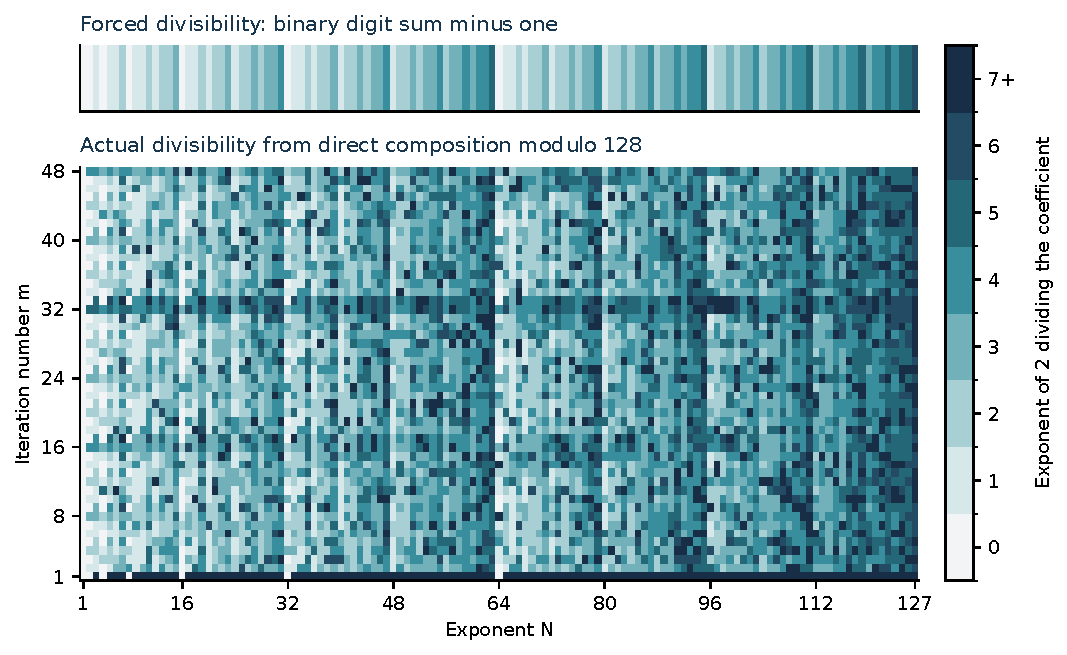
\includegraphics[width=\textwidth]{figures/02-digitsum-valuation_grid.pdf}
\caption{Exact binary divisibility in degrees $1\le N\le127$.
The upper strip is the uniform lower bound $s_2(N)-1$.
The lower panel shows $v_2(A_2(m,N))$ for $1\le m\le48$, capped
at seven. A value seven means divisibility by $128$; it includes
exact zero coefficients. The data come from direct ordinary-series
composition modulo $128$, without digit-based pruning. The theorem
explains the common forced layers, while the additional colors
record cancellations beyond the bound.}
\label{lim:dsd:fig:valuation}
\end{figure}

\section{Finite automata for each fixed iterate}
\label{lim:dsd:sec:automatic}

The sparse-support theorem does not itself provide all surviving
residues. A different argument gives a finite computation for every
coefficient modulo a fixed prime power, once the iterate is fixed.
We give the construction explicitly; it does not require the
characteristic-zero generating function to be algebraic or a
diagonal of a rational function.

\begin{definition}
For $0\le r<p$, the Cartier operator on $R[[x]]$ is
\begin{equation}
 \Lambda_r\left(\sum_{n\ge0}a_nx^n\right)
 =\sum_{n\ge0}a_{pn+r}x^n.
 \label{lim:dsd:eq:cartier}
\end{equation}
A sequence with values in a finite set is $p$-automatic if a finite
automaton with output reads the base-$p$ digits of its index and
returns the corresponding value.
\end{definition}

We use the least-significant-digit reading convention. The usual
equivalent characterization is finiteness of the $p$-kernel
\cite[Theorem 1.8]{dsdRY}. In the proof below, the automaton is built
directly from a finite Cartier-stable module.

\begin{lemma}[Lifting Frobenius]
\label{lim:dsd:lem:frobenius}
For $H(x)\in\Z[[x]]$ and $j\ge1$,
\begin{equation}
 H(x)^{p^j}\equiv H(x^p)^{p^{j-1}}\pmod{p^j}.
 \label{lim:dsd:eq:frobenius}
\end{equation}
Consequently, if $H(0)=0$ and $q\ge1$,
\begin{equation}
 F_p(H(x))\equiv
 \sum_{j=0}^{q-2}H(x)^{p^j}
 +\sum_{k\ge0}\left(H(x)^{p^{q-1}}\right)(x^{p^k})
 \pmod{p^q},
 \label{lim:dsd:eq:finite-power-reduction}
\end{equation}
where the first sum is empty for $q=1$.
\end{lemma}
\begin{proof}
The usual Frobenius congruence gives $H(x)^p\equiv H(x^p)\pmod p$.
If $U\equiv V\pmod{p^a}$ with $a\ge1$, the binomial expansion
shows $U^p\equiv V^p\pmod{p^{a+1}}$, including $p=2$.
Applying this $j-1$ times proves \eqref{lim:dsd:eq:frobenius}, the
congruence also used in the proof of \cite[Proposition 1.9]{dsdRY}.

For $j\ge q-1$, telescope \eqref{lim:dsd:eq:frobenius} at successive
substitutions and powers to obtain
\[
 H(x)^{p^j}\equiv
 H(x^{p^{j-q+1}})^{p^{q-1}}\pmod{p^q}.
\]
At $j=q-1$ this is an identity; for larger $j$ each discarded
difference is divisible by at least $p^q$. Summing yields
\eqref{lim:dsd:eq:finite-power-reduction}. The zero constant term makes
all infinite sums coefficientwise finite.
\end{proof}

\begin{lemma}[Two finite-module constructions]
\label{lim:dsd:lem:cartier-closure}
Let $R$ be a finite commutative ring.
\begin{enumerate}[label=\textup{(\roman*)}]
\item For every integer $k\ge1$, if a module with $d$ generators $u_1,\ldots,u_d$ is stable
under every $\Lambda_r$, then the module generated by
\begin{equation}
 x^c u_1^{\alpha_1}\cdots u_d^{\alpha_d},
 \quad 0\le c\le k-1,\quad \sum_i\alpha_i=k,
 \label{lim:dsd:eq:power-module}
\end{equation}
is Cartier-stable and contains $H^k$ for every $H$ in the original
module. It has at most $k\binom{d+k-1}{k}$ generators.
\item If $B(0)=0$ belongs to a finitely generated Cartier-stable
module, then adjoining
\begin{equation}
 \mathcal S(B)=\sum_{j\ge0}B(x^{p^j})
 \label{lim:dsd:eq:mahler-sum}
\end{equation}
gives another Cartier-stable module.
\end{enumerate}
\end{lemma}
\begin{proof}
Every series satisfies
$u(x)=\sum_{a=0}^{p-1}x^a(\Lambda_au)(x^p)$.
Apply this identity to the $k$ factors in a generator
\eqref{lim:dsd:eq:power-module}. A selected term has exponent
$c+a_1+\cdots+a_k$. Under $\Lambda_r$, it contributes only when
that exponent is $r$ modulo $p$, and its remaining power of $x$ is
\[
 \frac{c+a_1+\cdots+a_k-r}{p}\in\{0,\ldots,k-1\}.
\]
Each transformed factor is an $R$-linear combination of the $u_i$.
The result is therefore in the stated module. The count is the
number of degree-$k$ commutative monomials times the $k$ shifts.

For part (ii), put $C=\mathcal S(B)$. The identity
$C(x)=B(x)+C(x^p)$ gives
\begin{equation}
 \Lambda_0C=\Lambda_0B+C,\qquad
 \Lambda_rC=\Lambda_rB\quad(1\le r<p).
 \label{lim:dsd:eq:sum-transitions}
\end{equation}
Thus one additional generator suffices.
\end{proof}

\begin{theorem}[Constructive automaticity]
\label{lim:dsd:thm:automatic}
For every fixed prime $p$, precision $q\ge1$, and iterate $m\ge0$,
the sequence
\begin{equation}
 \bigl(A_p(m,N)\bmod p^q\bigr)_{N\ge0}
 \label{lim:dsd:eq:automatic-sequence}
\end{equation}
is $p$-automatic. For $m\ge1$, a Cartier representation with
$d_m$ generators can be constructed with $d_1=2$ and
\begin{equation}
 d_{m+1}\le1+\sum_{j=0}^{q-1}
 p^j\binom{d_m+p^j-1}{p^j}.
 \label{lim:dsd:eq:dimension-bound}
\end{equation}
Such a representation gives an automaton with at most $p^{qd_m}$
states and allows a coefficient query using
$O(d_m^2\log_p(N+1))$ ring operations after setup.
\end{theorem}
\begin{proof}
Work over $R=\Z/p^q\Z$. The module spanned by $1,F_p$ is stable:
\[
 \Lambda_0F_p=F_p,\quad \Lambda_1F_p=1,\quad
 \Lambda_rF_p=0\ (r\ge2).
\]
For the identity iterate, use the stable span of $1,x$ instead.
Starting from the representation of $F_p^{\circ m}$, apply
\cref{lim:dsd:lem:cartier-closure}(i) to each of the powers
$1,p,\ldots,p^{q-1}$ in \eqref{lim:dsd:eq:finite-power-reduction}.
Take the direct sum of those modules and adjoin the one Mahler-sum
generator from part (ii). This represents $F_p^{\circ(m+1)}$
and proves \eqref{lim:dsd:eq:dimension-bound}.

A module generated by $d_m$ elements over $R$ has at most
$|R|^{d_m}=p^{qd_m}$ elements. Its Cartier orbit is therefore
finite. Choose explicit transition matrices for the generators.
Starting at the vector representing $F_p^{\circ m}$, apply the
matrix for each successive least-significant digit of $N$.
The constant coefficient of the resulting series is $A_p(m,N)$.
This is a finite automaton with output. Dense matrix-vector
multiplication gives the stated operation bound; sparse matrices
are often much smaller.
\end{proof}

The construction is finite but its setup bound grows quickly with
$m$ and $q$. It is not a uniformly inexpensive algorithm in all
three parameters. Nor does substituting $m=N$ in the theorem
produce one finite automaton for the diagonal: the representation
would change with the input index.

The supplied implementation constructs sparse transition matrices,
without enumerating every automaton state. Four exact cross-checks
give the following unreduced representation sizes:
\begin{center}
\begin{tabular}{@{}rrrrr@{}}
\toprule
$p$ & $q$ & $m$ & Generators & Nonzero transition entries\\
\midrule
2&2&2&9&19\\
2&3&2&29&81\\
3&2&2&15&38\\
2&2&3&100&371\\
\bottomrule
\end{tabular}
\end{center}
These are sizes of the displayed construction, not minimal state
counts. They are independently verified through degree $512$ in
\texttt{data/cartier\_verification.json}.

\section{\texorpdfstring{$p$}{p}-adic iteration and periods in the iteration parameter}
\label{lim:dsd:sec:padic}

The main divisibility result also controls iteration at a $p$-adic
time. The construction below is classical finite-difference
interpolation applied coefficientwise; its useful additional
feature here is the digit-dependent divisibility of every
finite-difference coefficient.

Let $C$ be the linear substitution operator $C(H)=H\circ F_p$
on $\Q[[x]]$, and put $D=C-I$. Since $F_p=x+O(x^p)$,
\begin{equation}
 \ord_x(DH)\ge\ord_x(H)+p-1
 \quad\text{when }H\in x\Q[[x]],\ DH\ne0.
 \label{lim:dsd:eq:order-increase}
\end{equation}
This follows first for a monomial from
$F_p^j-x^j\in x^{j+p-1}\Z[[x]]$, then by linearity.

\begin{theorem}[A coefficientwise continuous iteration group]
\label{lim:dsd:thm:padic}
For $z\in\Z_p$, define
\begin{equation}
 F_p^{\circ z}(x)=\sum_{k\ge0}\binom zkD^kx.
 \label{lim:dsd:eq:padic-iteration}
\end{equation}
Each coefficient is a finite sum, belongs to $\Z_p$, and depends
continuously on $z$. The definition agrees with ordinary integer
iteration and satisfies
\begin{equation}
 F_p^{\circ(z+t)}=F_p^{\circ z}\circ F_p^{\circ t},\qquad
 F_p^{\circ0}=x,
 \qquad [x^p]F_p^{\circ z}=z.
 \label{lim:dsd:eq:padic-group}
\end{equation}
At a supported degree $N>1$, its coefficient has the form
\begin{equation}
 P_N(z)=\sum_{k=0}^{d_p(N)}b_{N,k}\binom zk,
 \qquad b_{N,k}\in p^{w_p(N)}\Z.
 \label{lim:dsd:eq:mahler-coefficients}
\end{equation}
Thus $P_N(z)\in p^{w_p(N)}\Z_p$ for every $z\in\Z_p$.
\end{theorem}
\begin{proof}
The order increase \eqref{lim:dsd:eq:order-increase} proves coefficientwise
finiteness and the degree bound in \eqref{lim:dsd:eq:mahler-coefficients}.
For a nonnegative integer $m$, the finite binomial identity
$(I+D)^m=C^m$ gives ordinary iteration.

At degree $N>1$,
\begin{equation}
 b_{N,k}=[x^N]D^kx
 =\sum_{j=0}^k(-1)^{k-j}\binom kj A_p(j,N).
 \label{lim:dsd:eq:finite-difference}
\end{equation}
Every term is divisible by $p^{w_p(N)}$ by \cref{lim:dsd:thm:main};
the identity-iterate term is zero. This proves the asserted
divisibility of the finite differences.

The polynomial $\binom zk$ maps $\Z_p$ into $\Z_p$: it is
continuous over $\Q_p$, and its integer values on the dense set
of nonnegative integers are $p$-integral. Hence every coefficient
in \eqref{lim:dsd:eq:padic-iteration} is continuous and $p$-integral.
For each fixed degree, composition uses finitely many coefficient
polynomials in $z,t$. The group identity holds on pairs of
nonnegative integers and extends by continuity to $\Z_p^2$.
It identifies negative integers with formal inverse iteration.
Finally, $Dx$ has coefficient one at $x^p$, and $D^kx$ has no
such term for $k\ge2$, proving the last identity.
\end{proof}

The continuity here is in the \emph{coefficientwise $p$-adic}
topology, not the pure $x$-adic topology. For example, a small
nonzero $p$-adic parameter still produces the term $zx^p$.
The parameterization is injective because that coefficient
recovers $z$. Also, $P_N(z)$ is an integer-valued rational
polynomial; it need not be a polynomial in $\Z[z]$.

\begin{theorem}[A digit-sensitive sufficient period]
\label{lim:dsd:thm:period}
Let $N>1$ be supported, $d=d_p(N)$, $w=w_p(N)$, and $q\ge1$.
If $q\le w$, then $P_N$ is identically zero modulo $p^q$.
If $q>w$, its value modulo $p^q$ depends only on
\begin{equation}
 z\pmod{p^h},\qquad h=q-w+\lfloor\log_p d\rfloor.
 \label{lim:dsd:eq:period}
\end{equation}
No minimality of this period is asserted.
\end{theorem}
\begin{proof}
Only the case $q>w$ needs proof. Then $p^h>d$. For
$1\le i\le d$,
\begin{equation}
 v_p\binom{p^h}{i}=h-v_p(i)\ge q-w.
 \label{lim:dsd:eq:binomial-period-valuation}
\end{equation}
Indeed, $\binom{p^h}{i}=(p^h/i)\binom{p^h-1}{i-1}$,
and the second factor is a $p$-adic unit, as is seen by
reducing $(1+X)^{p^h-1}$ modulo $p$.
Vandermonde's identity gives
\[
 \binom{z+p^h}{k}-\binom zk
 =\sum_{i=1}^k\binom{p^h}{i}\binom z{k-i}.
\]
Multiplying by $b_{N,k}\in p^w\Z$ and summing proves
$P_N(z+p^h)\equiv P_N(z)\pmod{p^q}$. Integer multiples
follow by iteration; all $p$-adic multiples follow by continuity.
\end{proof}

The degree-one coefficient is identically one and needs no period
formula. Unsupported coefficients are identically zero. The period
estimate can be far from minimal, particularly at a pure-power
degree, where \eqref{lim:dsd:eq:modp-row} already gives a smaller
description modulo $p$.

\section{Exact computations and reproducibility}
\label{lim:dsd:sec:verification}

Every unbounded assertion above rests on its written proof. The
programs serve as independent checks of formulas, indexing,
normalization and implementation. They use exact integer or
finite-ring arithmetic; the plotting dependencies are matplotlib and NumPy.

\subsection{Three independent computational routes}

\texttt{code/verify.py} directly composes ordinary power series
without discarding coefficients on the basis of the digit theorem.
It checks support and divisibility for $p=2,3,5,7$, iterates
$1\le m\le8$ and degrees through $128$, and checks inverse
series through degree $35$. Separately, it implements the
set-partition Bell recurrence and compares the scaled coefficients
with ordinary composition through degree $28$. It also checks
the Fuss--Catalan valuation, the first ten terms of each of the
three OEIS diagonals, the odd-prime examples, and sufficient periods.

\texttt{code/leading\_residue.py} constructs the digit polynomial
over $\Fp$ using a sparse dictionary. Its verifier compares against
a separate ordinary-composition routine for all degrees $0$ through
$300$ and $p=2,3,5,7$. It additionally checks highest-digit stability
and the three sharp families.

\texttt{code/cartier.py} implements the finite-module construction
from \cref{lim:dsd:sec:automatic}. Its verifier compares coefficient queries
against direct Cauchy composition through degree $512$ in four
parameter settings. It can also export the sparse transition
representation as JSON. It guards against excessive setup sizes;
these guards are resource limits, not restrictions of the theorem.

\begin{center}
\small
\begin{tabular}{@{}L{0.57\textwidth}r@{}}
\toprule
Recorded independent check & Number\\
\midrule
Coefficient support, valuation, and scaled integrality & 4236\\
Ordinary composition versus Bell composition & 336\\
Exact Fuss--Catalan valuations & 750\\
OEIS initial-term fixtures & 30\\
Digit formula versus ordinary second composition & 1204\\
Highest-digit stability comparisons & 70\\
Sharp-family evaluations & 18\\
Cartier queries versus ordinary composition & 2052\\
\bottomrule
\end{tabular}
\end{center}

The counts above describe finite checks, not a count of proved
theorems. Exact receipts are supplied in the \texttt{data/} directory.
The heatmap uses another direct modular composition calculation.
No numerical fit, floating-point valuation, or guessed recurrence
is used in any proof.

\subsection{Reproduction commands}

From the package directory, run:
\begin{verbatim}
python3 code/verify.py --output data/verification.json \
    --heatmap data/valuation_grid.json
python3 code/leading_residue.py \
    --verify data/leading_residue_verification.json
python3 code/cartier.py --verify \
    --verification-output data/cartier_verification.json
python3 code/make_figure.py
pdflatex -interaction=nonstopmode -halt-on-error article.tex
pdflatex -interaction=nonstopmode -halt-on-error article.tex
\end{verbatim}
The first and second commands explicitly name their output files.
The Cartier verifier's output path and query options are documented
by its \texttt{--help} output and in \texttt{README.txt}.
The supplied figure PDF permits compilation without matplotlib.

\emph{[Write note, batch 114, 6 October 2026.]} These are the commands of the delivered layout. In
this report the files carry the prefix \texttt{02-digitsum-}
(\cref{lim:dsd:tab:files}); \texttt{make\_figure.py} reads and writes fixed
delivery paths under its parent directory, the other programs write where
they are told, and on Windows they write CRLF line endings. Run them on a
copy in the delivered layout, never in place; the README gives the route,
and \cref{lim:dsd:sec:intake} reports the intake's rerun.

\section{Source audit and limits of the conclusions}
\label{lim:dsd:sec:audit}

The inspected repository article is
\begin{quote}\small
\nolinkurl{SetTheory/Cardinals/docs/reports/congruences-and-valuations/}\\
\nolinkurl{iterated-series/a168362-lacunary-iterates-mod4/article.tex}.
\end{quote}
Its Git blob is
\nolinkurl{46147fca8f8fb912f7132d504b21217c0c248844}.
That exact blob was verified at repository commit
\nolinkurl{3412ae0741b95b3fb6d7a43477b7fac7723c36d8}.
The snapshot was inspected on October 5, 2026. Its Questions 13.2
and 13.3 are the direct targets of this article.

The repository's report on compositional tree-series congruences
studies different labeled-tree exponential generating functions.
Its wider-class discussion does not include arbitrary ordered
arity restrictions. A sibling on self-iterating series uses
negative iterates and $p$-adic iteration in another functional
equation. These are relevant methodological neighbors, not
sources for the present lacunary digit bound. The iterated-Bell
diagonal report contains an analytic method pointer for A168362,
without asserting its ratio conjecture.

The external checks covered the current OEIS definitions and
comments, the Hurwitz-series composition reference \cite{dsdBCM},
and the prime-power Cartier and automaton framework \cite{dsdRY}.
Targeted searches for the exact sequence and for lacunary
composition with digit-sum divisibility did not locate the
present application. This is a bounded search result, not a
proof of publication priority. The classical tools are derived
in the article, so no unverified repository claim is a proof
dependency.

The important limitations are mathematical and specific:
\begin{itemize}
\item The digit cutoff is a necessary support condition. Extra
divisibility and cancellation are common. Except for the explicit
second-iterate formula and families, no equality classification
for the valuation is asserted.
\item Universal optimality is proved in $\Cp^1$ through the inverse
of $x+x^p$. For the particular full $F_p^{\circ2}$, only the
stated weights one, two and three are proved sharp in infinite
families here.
\item Automaticity is proved for each fixed nonnegative integer
iterate and fixed precision. No automaticity claim is made for
the diagonal $m=N$, for arbitrary $p$-adic time, or for negative
iterates modulo higher prime powers.
\item The period in \cref{lim:dsd:thm:period} is sufficient and may be
large. The setup costs of the automaton construction can also
grow rapidly.
\item The source report's real asymptotic ratio question is
unresolved by these congruence arguments. The previous exact
modulo-four diagonal classification and its counting constant
are not re-proved or claimed as new.
\end{itemize}

\emph{[Write note, batch 114, 6 October 2026.]} The pinned blob is Part~I as printed here, without
its notes of 6~October 2026 (\cref{lim:dsd:sec:provenance}). The statements
above about the neighbouring reports were checked and are correct:
\texttt{compositional-tree-series-congruences} says that its wider class of
tree specifications does not include arbitrary degree restrictions or
ordered children; \texttt{a396807-self-iterating-series} treats iterates of
every integer order and $p$-adic-time iteration of its own series; and
\texttt{a139383-iterated-bell-diagonals} names Part~I's refined asymptotic
as open and makes no claim about it. The ``two independent mathematical
reviews'' of the source audit are, by the delivered
\texttt{data/document\_qa.json}, two AI audits; this is a process claim the
intake cannot verify. No human review and no formal verification is
claimed.

\section{Further research questions and proposed approaches}
\label{lim:dsd:sec:questions}

The following questions arise from the results proved here. Their
status refers to this article and the inspected sources, rather
than an exhaustive claim about all literature.

\emph{[Write note, batch 114, 6 October 2026.]} Under Vladimir Reshetnikov's standing rule of
4~October 2026, unproved claims are kept as open questions. These ten are
the manuscript's, with its proposed approaches; the write found no other
unproved claim in it and no statement of it to be wrong. Research
question~\ref{lim:dsd:q:ratio} restates Part~I's Research
question~\ref{lim:q:ratio}; Research question~\ref{lim:dsd:q:diagonals}
continues Research question~\ref{lim:q:higher-precision} on the diagonal,
where the iteration index moves with $N$; Research
question~\ref{lim:dsd:q:higher-residues} continues the re-scoped Research
question~\ref{lim:q:odd-prime}.

\begin{question}[Exact higher-modulus diagonals]
\label{lim:dsd:q:diagonals}
Classify $A_2(N,N)\bmod8$ and $\bmod16$, including the surviving
three- and four-bit layers, and obtain the sharp count of nonzero
indices below $X$.
\end{question}
The new filtration removes all larger-weight indices, but the
iteration number is still $N$. A useful approach is to combine
finite differences in the iteration parameter with a carry
calculus restricted to the finitely many permitted digit layers.
The earlier modulo-four diagonal classification gives a stringent
specialization check.

\begin{question}[Arbitrary-depth sharpness for the full second iterate]
\label{lim:dsd:q:sharpness}
For every $p$ and every $w\ge4$, does some degree $N$ satisfy
$v_p(A_p(2,N))=w_p(N)=w$? Can one give uniform infinite families?
\end{question}
By highest-digit stability, one example at a given digit pattern
immediately gives infinitely many. The remaining problem is to
find a pattern whose digit-polynomial functional in
\eqref{lim:dsd:eq:residue} is nonzero. The Fuss--Catalan example does not
answer this more specific question.

\begin{question}[Leading residues of higher iterates]
\label{lim:dsd:q:higher-residues}
Find a digit-level formula for $A_p(m,N)/p^{w_p(N)}\bmod p$
for general fixed $m$, comparable to \cref{lim:dsd:thm:residue}.
\end{question}
Repeated Bell composition suggests a hierarchy of carry-free
digit allocations. A successful formula should keep the number
of states controlled in $m$ and the digit weight, rather than
enumerate all labeled set partitions of $N$.

\begin{question}[Minimal Cartier representations]
\label{lim:dsd:q:cartier-min}
Determine the minimal automaton or minimal linear representation
for selected $(p,q,m)$, and improve \eqref{lim:dsd:eq:dimension-bound}.
\end{question}
The current construction deliberately keeps dependent generators.
Finite-ring relations among its shifted monomials can make the
actual representation much smaller. Over $\Z/p^q\Z$, reduction
must respect nonunits; field Gaussian elimination alone is not
a general minimization procedure.

\begin{question}[Inverse-iterate automaticity]
\label{lim:dsd:q:inverse-auto}
Are the coefficient sequences of $F_p^{\circ(-m)}$ modulo $p^q$
$p$-automatic for every fixed positive $m,q$?
\end{question}
The valuation theorem and $p$-adic period theorem cover these
iterates, while the finite forward-composition construction does
not. An effective inverse closure theorem adapted to the
Mahler-sum representation would connect the two parts of the paper.

\begin{question}[Optimal iteration periods]
\label{lim:dsd:q:periods}
Determine the least period of $A_p(m,N)\bmod p^q$ as a function of $m$.
Describe this period from the base-$p$ digits of $N$.
\end{question}
The sufficient period comes from bounding all binomial terms by
their maximum degree. The valuations and cancellations of the
individual finite differences $b_{N,k}$ should often improve it.
Pure-power degrees give accessible exact test cases.

\begin{question}[Typical excess valuation]
\label{lim:dsd:q:excess}
For fixed $m$, or for $m=N$, study
$v_p(A_p(m,N))-w_p(N)$ at nonzero coefficients and determine
its distribution over digit strings.
\end{question}
The current density-one theorem supplies only the forced part.
For a fixed row the finite automaton can support exact frequency
calculations at each modulus. Passing to all precisions or to a
moving diagonal requires additional uniform control.

\begin{question}[Which weighted seeds retain automaticity?]
\label{lim:dsd:q:weighted-auto}
For $W(x)=x+\sum b_jx^{p^j}$, characterize the coefficient
sequences $(b_j)$ for which fixed iterates of $W$ are
$p$-automatic modulo each $p^q$.
\end{question}
The divisibility theorem allows arbitrary integer weights.
Automaticity is more restrictive: already the seed can encode
an arbitrary sequence along the powers of $p$. Eventually
periodic weights in the exponent index provide a natural first
class with finite Mahler systems.

\begin{question}[The real-growth diagonal problem]
\label{lim:dsd:q:ratio}
Prove or refute the recorded conjecture
$A_2(N+1,N+1)/A_2(N,N)\sim eN$, and determine a multiplicative
asymptotic for the diagonal if it holds.
\end{question}
The ordered level-tree interpretation gives a concrete counting
model. The present divisibility results impose arithmetic
constraints but do not estimate the sizes of its positive
coefficients. A saddle-point or branching analysis must also
handle the fact that depth and leaf count grow together.

\begin{question}[Formal verification]
\label{lim:dsd:q:formal}
Formalize the digit-divisibility theorem with the smallest
reusable mathematical interface.
\end{question}
The proof separates naturally into factorial valuation, integral
set-partition composition, and the weighted scaling identity.
The core theorem needs no analytic estimates or automata library.
A second stage could verify the digit-polynomial formula and
finite transition certificates for concrete automata.

\emph{[Independent check of the write, 6 October 2026.]} An adversarial
check made by the intake after the write (commit \texttt{42d31831e}), with
its own exact integer code, found every addition of the write correct. It
confirmed the counterexample to Research question~\ref{lim:q:odd-prime}
(\cref{lim:dsd:prop:odd-correction}; $[x^{2p-1}]F_p(F_p(x))=p$ computed for
all primes $p\le13$) and the corrected support statement modulo~$p^2$ (the only
digit sums carrying a coefficient nonzero modulo~$p^2$ are $1$ and $p$, and
$p$ is occupied for every tested $m\notin\{0,1\}$, inverse iterates
included); the answer to Research question~\ref{lim:q:higher-precision} for
every $q$, with the support condition, the valuation bound and the
integrality of $N!\,A_p(m,N)/p^{(N-1)/(p-1)}$ holding at $4090$ coefficients
($p\le11$, $-3\le m\le6$); the second routes to
\cref{lim:thm:whole-array-support}, to \cref{lim:prop:P-closed}
(\eqref{lim:dsd:eq:modp-row} in $170$ of $170$ cases) and to
\cref{lim:prop:diagonal-even} ($p\mid A_p(N,N)$ for $2\le N\le40,30,26$ at
$p=2,3,5$); \cref{lim:dsd:rem:oeis-example} against the live entries (the
printed rows of A168365, A168366 and A168362, $114$, $110$ and $64$
entries, are those of plain composition); the agreement at $p=2$, $m=2$
with \cref{lim:thm:full-array-formula}(c),(d) claimed in
\cref{lim:dsd:sec:claims} (its own implementation of the residue formula of
\cref{lim:dsd:thm:residue} agrees with direct composition in $160$, $60$,
$32$ and $17$ cases for $p=2,3,5,7$); and the \verb|\crefalias| change
(Part~I's heads, equation tags and appendix letters unchanged; the nine
cross-references of the earlier build that named a lemma, proposition or
corollary ``Theorem'' now carry the right name; no undefined reference). A
minor observation, needing no change: A168366's example prints no $F_0$
row, so the initial condition $F_0(x)=x$ in
\cref{lim:dsd:rem:oeis-example} is the natural one there, not a printed
one. The check also found an error of Part~I that predates the write:
formula~\eqref{lim:eq:array-power-formula} of
\cref{lim:thm:full-array-formula}(c) is false with its binomial read as an
integer. Under the standing rule of 4~October 2026 it is kept as printed
and corrected, with the counterexample, in a dated note after the proof of
that theorem; Part~II uses only its content modulo~$2$.

\appendix
\phantomsection
\addcontentsline{toc}{part}{Appendices}
\part*{Appendices}

\emph{[Write note, batch 114, 6 October 2026.]} Appendices~A and~B belong to Part~I;
Appendices~\ref{lim:dsd:app:oeis-note} and~\ref{lim:dsd:app:inventory}
belong to Part~II.

\section{Proposed OEIS update text}

The following is a concise draft, not submitted to OEIS.

\begin{quote}\small
Let $F(x)=\sum_{j\ge0}x^{2^j}$ and $a(n)=[x^n]F^{\circ n}(x)$.  For $s\ge1$
put $M_s=2^s-1$ and define $R_s\subseteq\mathbb Z/2^s\mathbb Z$ by
\[
\ind_{d\in R_s}\equiv\ind_{d=0}+
\sum_{i=0}^s\ind_{i\,\mathrm{OR}\,((i+d)\bmod2^s)=M_s}\pmod2.
\]
Then $a(n)$ is even for every $n>1$.  Moreover, $a(n)\equiv2\pmod4$ exactly
for $n\in\{2,3,4,6\}$ and for
$n=2^r+2^s$ with $r>s\ge1$, $r\ge3$, and
$r-s\bmod2^s\in R_s$; all other $n>1$ give $a(n)\equiv0\pmod4$.
The next exceptional indices after the currently listed $520$ are
$1028,1032,2056,2064,4100,4104,\ldots$.  If $E(X)$ counts the exceptions up
to $X$, then
$E(X)=\kappa\log_2X+O((\log\log X)^3)$, where
$\kappa=\sum_{s\ge1}|R_s|/2^s=2.323930059308106\ldots$.
\end{quote}

\section{Artifact inventory}
\label{lim:app:inventory}

\emph{[Write note, batch 73O1.]} In the collection, \texttt{article.tex}
is the delivered source with prefixed labels and these notes,
\texttt{article.pdf} is a build of it, and \texttt{README.md} is the
collection README;
the delivered PDF and README, a file list \texttt{MANIFEST.txt} and the
checksum list \texttt{SHA256SUMS.txt} are not shipped. The other files
below are shipped under the names shown, byte-identical to the delivery.


The accompanying archive contains:
\begin{center}
\begin{tabular}{ll}
\toprule
File & Purpose\\
\midrule
\texttt{article.tex}, \texttt{article.pdf} & manuscript source and compiled PDF\\
\texttt{code/verify\_a168362.py} & exact standard-library verifier\\
\texttt{data/verification.json} & machine-readable PASS record\\
\texttt{data/verification\_run.txt} & complete verifier stdout\\
\texttt{data/residue\_sets.csv} & $R_s$ for $1\le s\le64$\\
\texttt{data/exceptional\_indices\_to\_10m.txt} & exceptions through $10^7$\\
\texttt{oeis\_update\_draft.txt} & plain-text version of the proposed update\\
\texttt{README.md} & build and verification instructions\\
\bottomrule
\end{tabular}
\end{center}

\section{A concise theorem suitable for an OEIS note}
\label{lim:dsd:app:oeis-note}

The following text is a draft for mathematical review, not a
record of a submission.

\emph{[Write note, batch 114, 6 October 2026.]} Nothing was submitted to OEIS. Part~I's
Appendix~A is a draft of the same kind for the modulo-four theorem.

\begin{quote}
Let $F(x)=\sum_{j\ge0}x^{2^j}$. For every integer $m$ and
$N\ge1$, the coefficient $[x^N]F^{\circ m}(x)$ is divisible by
$2^{s_2(N)-1}$, where $s_2(N)$ counts the ones in the binary
expansion of $N$; negative $m$ denotes compositional inversion.
In particular A168362, A168365 and A168366 are divisible by
$2^q$ whenever $s_2(N)>q$. The assertion follows by observing
that $\sum_{j\ge0}x^{2^j}/2^{2^j-1}$ has integer exponential
coefficients and that this property is preserved by composition
and inversion. Legendre's formula then gives the stated exponent.
\end{quote}

\section{Package inventory}
\label{lim:dsd:app:inventory}

The article is self-contained apart from its supplied figure.
The ZIP contains the following principal files:
\begin{center}
\small
\begin{tabular}{@{}L{0.43\textwidth}L{0.5\textwidth}@{}}
\toprule
File & Purpose\\
\midrule
\texttt{article.tex}, \texttt{article.pdf} & Complete source and compiled article\\
\texttt{README.txt} & Build instructions and example queries\\
\texttt{SOURCE\_AUDIT.txt} & Source pin, provenance and novelty boundaries\\
\texttt{code/verify.py} & Ordinary and Bell composition; inverse, valuation and period checks\\
\texttt{code/leading\_residue.py} & Exact sparse first-residue algorithm\\
\texttt{code/cartier.py} & Sparse finite-module construction and coefficient queries\\
\texttt{code/make\_figure.py} & Recreates the scientific figure\\
\texttt{data/} & Exact verification receipts and figure data\\
\texttt{figures/valuation\_grid.pdf} & Vector figure used by the article\\
\bottomrule
\end{tabular}
\end{center}

\emph{[Write note, batch 114, 6 October 2026.]} Of these, \texttt{article.tex}, \texttt{article.pdf}
and \texttt{README.txt}, and the checksum list \texttt{SHA256SUMS.txt}, are
not shipped; the others are shipped under the names of
\cref{lim:dsd:tab:files}, with \texttt{data/document\_qa.json} and
\texttt{figures/valuation\_grid.png}.

\begin{thebibliography}{99}

\bibitem{OEIS-A168362}
P. D. Hanna,
\emph{A168362: coefficient of $x^n$ in the $n$-th iteration of
$\sum_{k\ge0}x^{2^k}$},
The On-Line Encyclopedia of Integer Sequences,
\url{https://oeis.org/A168362}, accessed October 1, 2026.

\bibitem{OEIS-A168365}
P. D. Hanna,
\emph{A168365: coefficient of $x^n$ in the $(n-1)$-st iteration of
$\sum_{k\ge0}x^{2^k}$},
OEIS, \url{https://oeis.org/A168365}.

\bibitem{OEIS-A168366}
P. D. Hanna,
\emph{A168366: coefficient of $x^n$ in the $(n+1)$-st iteration of
$\sum_{k\ge0}x^{2^k}$},
OEIS, \url{https://oeis.org/A168366}.

\bibitem{OEIS-A112317}
P. D. Hanna,
\emph{A112317: coefficients of $x^n$ in the $n$-th iteration of $x+x^2$},
OEIS, \url{https://oeis.org/A112317}.

\bibitem{OEIS-A122888}
P. D. Hanna and contributors,
\emph{A122888: coefficient triangle for iterates of $x+x^2$},
OEIS, \url{https://oeis.org/A122888}.

\bibitem{OEIS-A086753}
J. Perry and contributors,
\emph{A086753: number of distinct entries in a trinomial slice},
OEIS, \url{https://oeis.org/A086753}.

\bibitem{Fine1947}
N. J. Fine,
\emph{Binomial coefficients modulo a prime},
American Mathematical Monthly \textbf{54} (1947), 589--592.

\bibitem{StanleyEC1}
R. P. Stanley,
\emph{Enumerative Combinatorics, Volume 1}, second edition,
Cambridge University Press, 2012.

\bibitem{FlajoletSedgewick}
P. Flajolet and R. Sedgewick,
\emph{Analytic Combinatorics},
Cambridge University Press, 2009.

\bibitem{ProveIt}
V. Reshetnikov,
\emph{ProveIt: formal mathematics and reproducible research artifacts},
\url{https://github.com/VladimirReshetnikov/ProveIt},
repository inspected October 1, 2026.

\bibitem{dsdrepo}
V. Reshetnikov, \emph{ProveIt repository}, research-report collection.
\emph{Binary Carry Structure in Iterated Lacunary Series},
October 1, 2026, especially Questions 13.2--13.3.
\url{https://github.com/VladimirReshetnikov/ProveIt}.
Exact path, commit and file blob are recorded in \cref{lim:dsd:sec:audit}
and \texttt{SOURCE\_AUDIT.txt}. The earlier report is an
AI-assisted, unrefereed manuscript.
[Write note, batch 114: this is Part~I of the present report.]

\bibitem{dsdBCM}
S. Barbero, U. Cerruti and N. Murru,
\emph{On the operations of sequences in rings and binomial type sequences},
Ricerche di Matematica (2018),
\href{https://doi.org/10.1007/s11587-018-0389-5}{doi:10.1007/s11587-018-0389-5}.
\url{https://arxiv.org/abs/1805.11922}.
The subsection on compositions of generating functions is the
background reference for Hurwitz-series composition and inversion.

\bibitem{dsdRY}
E. Rowland and R. Yassawi,
\emph{Automatic congruences for diagonals of rational functions},
Journal de th\'eorie des nombres de Bordeaux \textbf{27} (2015),
245--288,
\href{https://doi.org/10.5802/jtnb.901}{doi:10.5802/jtnb.901}.
\url{https://jtnb.centre-mersenne.org/item/10.5802/jtnb.901.pdf}.
Theorem 1.8 and Proposition 1.9 provide the standard kernel
criterion and prime-power congruence discussed in
\cref{lim:dsd:sec:automatic}; their rational-diagonal hypotheses are not
assumed for the lacunary series here.

\end{thebibliography}

\end{document}
